% !TeX root = ../main.tex
\chapter{Project 06: Distributed Control of a Multi-agent magnetic levitation system}

\section{Objectives}
The aim of this project is analyze the effect of different network structures and control parameters on the cooperative control protocol and the global observer, and finally designing a control protocol and observer to reach consesnsus among the nodes - choosing a network structure among different possible topologies.

\section{Setting of the problem}
\subsection{Dynamics of the Nodes}
The system under study comprises of 7 almost identical magnetic levitation system, of which one is chosen as leader node and others followers. The dynamic of each node is described as follows:


\begin{align*}
\dot{x}_i &= A x_i + B u_i \\
y_i &= C x_i
\end{align*}

with matrices:

\[
A = \begin{bmatrix}
0 & 1 \\
880.87 & 0
\end{bmatrix}, \quad
B = \begin{bmatrix}
0 \\
-9.9453
\end{bmatrix}, \quad
C = \begin{bmatrix}
708.27 & 0
\end{bmatrix}, \quad
D = \begin{bmatrix}
0
\end{bmatrix}
\]

Regarding the observability and controllability of each node, it can be easily investigated that both states of the nodes are observable and controllable. However, as it can be seen only the first state of the system is measured, and an observer, global or local, needs to be used for the perpuse of \textit{State-variable feedback control}. 

The fundamental assumptions regarding the whole system is as follows:
\begin{enumerate}
	\item The leader node $S_0$ can be observed by a small subset of the follower nodes
	\item The controller law of each aget can only enjoy the information of the neighbor nodes
	\item There exists at lead one directed path from the leader node to every follower node.
\end{enumerate}

\subsection{Reference generation by the leader node}
As the nodes are unstable, in order for the leader to generate a reference signal: first, a local observer needs to be adopted for the leader node, and then, a local controller needs to be adopted to perform the eigenvalue placement depending on the desired reference to be generated. For each desired signal, the eigvenvalues of the leader should be placed as follows:
\begin{itemize}
	\item Step reference: [0 , -$\lambda$], with impact input 
	\item Ramp reference: [0, 0], with impact input
	\item Sinusoidal: [+$\omega$j,  -$\omega$j], with impact input
\end{itemize}

In our case, for the sake of conformity of the different tests, these values are chosen as follows:
\begin{itemize}
	\item Step reference: [0 , -5], with impact input 
	\item Ramp reference: [0, 0], with impact input
	\item Sinusoidal: [+j,  -j], with impact input
\end{itemize}

And for the local observer, -10 and -15. In a noise-free case, it is more desirable to choose faster eigenvalue for the observer; this, nonetheless, leads to worsening the performance in an noisy environment, or in the case of using cheap sensors. Therefore, the eigenvalues of the observer should not be chosen to be much large than the eigenvalues of the plant.

Since by the assumption all the nodes need to be identical, the same controller must be used on all the nodes.

The plots of the references generated by the leader are as follows:
\begin{figure}[H] % h means "here", can also use t (top), b (bottom), p (page)
    \centering
    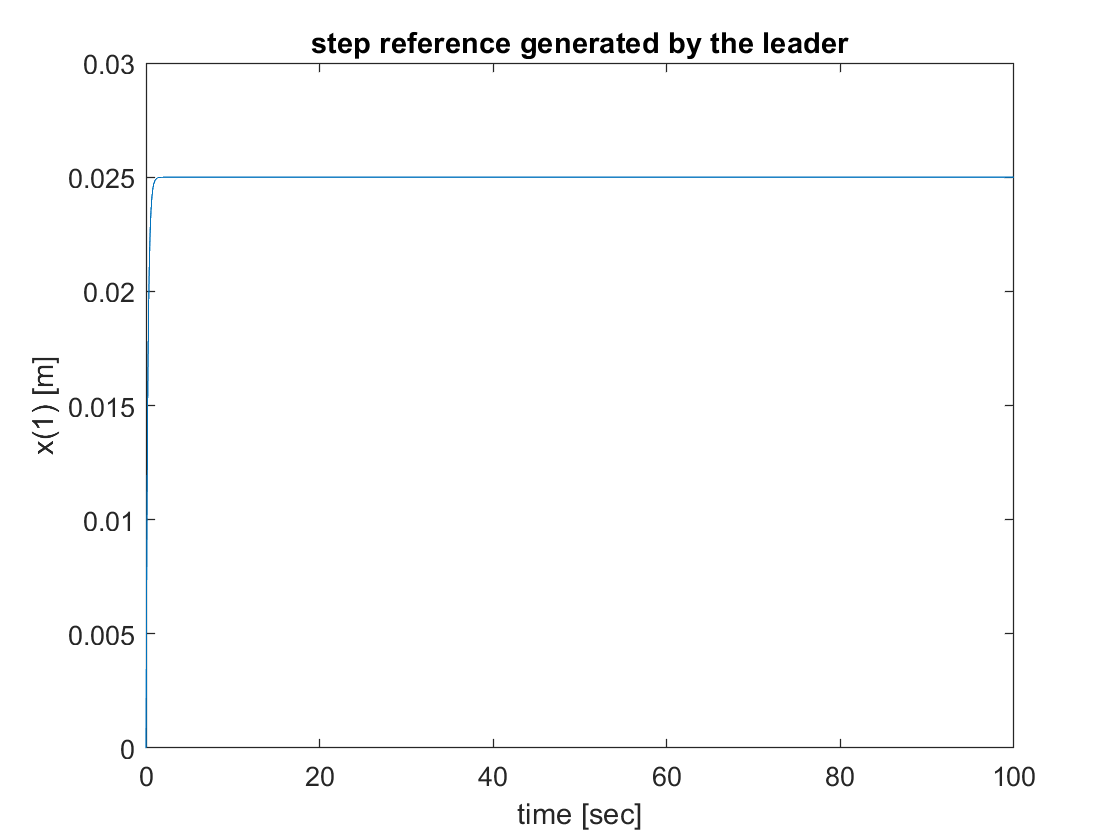
\includegraphics[width=0.55\textwidth]{step_reference.png} % Adjust width as needed
    \caption{Step reference generated by the leader load.}
\end{figure}

\begin{figure}[H] % h means "here", can also use t (top), b (bottom), p (page)
    \centering
    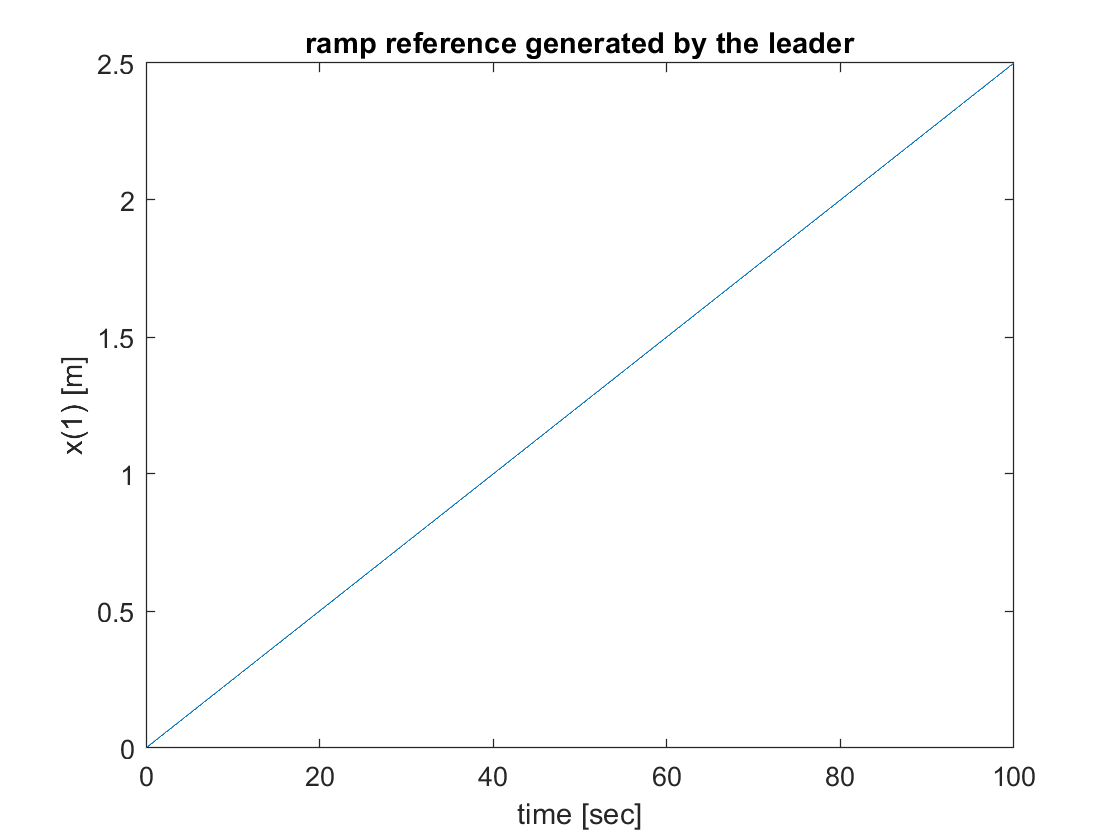
\includegraphics[width=0.55\textwidth]{ramp_reference.png} % Adjust width as needed
    \caption{Ramp reference generated by the leader load.}
\end{figure}

\begin{figure}[H] % h means "here", can also use t (top), b (bottom), p (page)
    \centering
    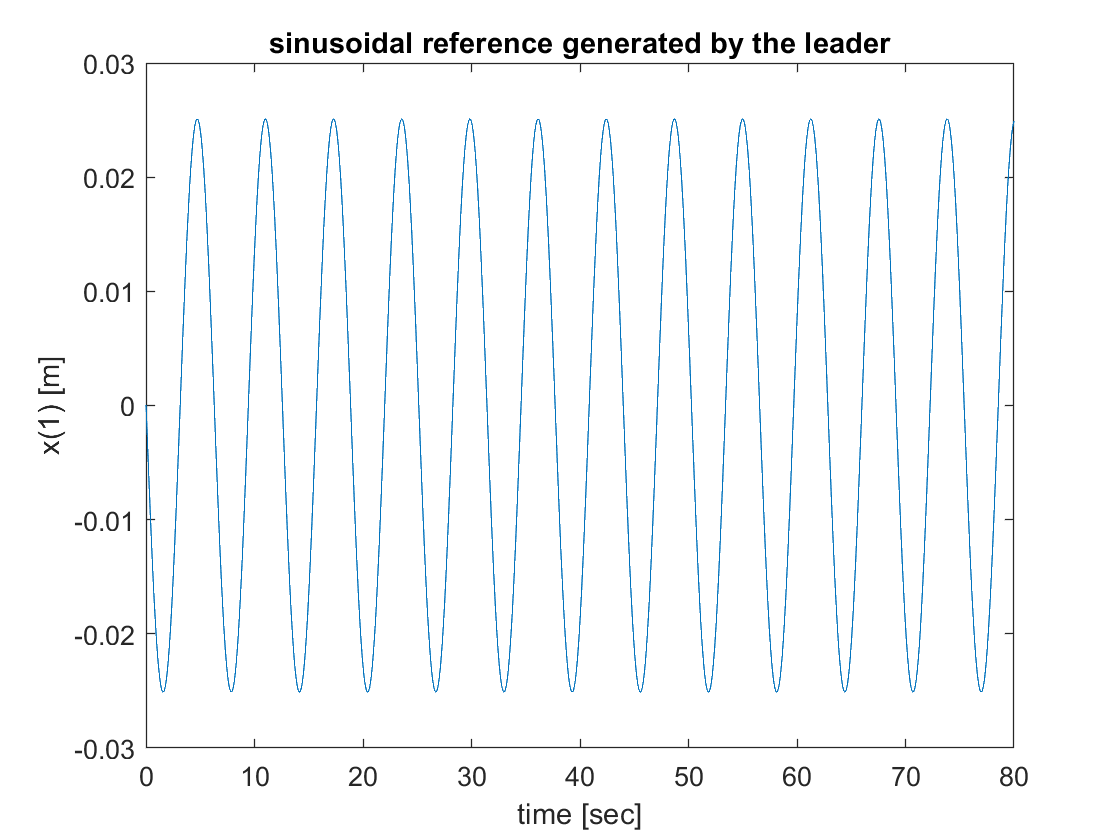
\includegraphics[width=0.55\textwidth]{sinusoildal_reference.png} % Adjust width as needed
    \caption{Sinusoidal reference generated by the leader load.}
\end{figure}


\subsection{Simulation Equation}
For the purpose of simulation, the global dynamics is used, and then the plots are made seperating the relavant states of each nodes. For the case where the local observer are used for the nodes. The state equations used are as follows:


\begin{align*}
A_c &= I_N \otimes A - c_c (L_{\text{cal}} + G_{\text{cal}}) \otimes BK \\
B_c &= c_c (L_{\text{cal}} + G_{\text{cal}}) \otimes BK \\
C_c &= I_{Nn} \\
D_c &= \mathbf{0}_{Nn \times Nn}
\end{align*}

where:
\begin{itemize}
  \item $N$ is the number of agents (excluding the leader),
  \item $n$ is the dimension of the individual agent state (considering the local observer, twice as large as the original $n$),
  \item $A$, $B$ are the agent system modified matrices (the closed-loop node with the controller and the observer),
  \item $K$ is the state feedback gain,
  \item $c_c$ is the coupling gain,
  \item $L_{\text{cal}}$ is the Laplacian matrix of the agent graph,
  \item $G_{\text{cal}}$ is the pinning matrix,
  \item $\otimes$ denotes the Kronecker product.
\end{itemize}

Here, the matrix $C$ is used in this manner so that after the simulation we get all the states of the system.

In case of distributed observer, the following system should be used, where the states vector is the stack of original states and the observer states.

\begin{align*}
A_o &= I_N \otimes A - c_o (L_{\text{cal}} + G_{\text{cal}}) \otimes F C \\
A_c &= 
\begin{bmatrix}
I_N \otimes A & -c_c (L_{\text{cal}} + G_{\text{cal}}) \otimes B K \\
c_o (L_{\text{cal}} + G_{\text{cal}}) \otimes F C & 
A_o - c_c (L_{\text{cal}} + G_{\text{cal}}) \otimes B K
\end{bmatrix} \\
B_c &= 
\begin{bmatrix}
c_c (L_{\text{cal}} + G_{\text{cal}}) \otimes B K \\
c_c (L_{\text{cal}} + G_{\text{cal}}) \otimes B K
\end{bmatrix} \\
C_c &= I_{2Nn} \\
D_c &= \mathbf{0}_{2Nn \times Nn}
\end{align*}

where:
\begin{itemize}
  \item $N$ is the number of agents,
  \item $n$ is the dimension of each agent's state,
  \item $A$, $B$, $C$ are the agent's system matrices,
  \item $K$ is the state feedback gain ,
  \item $F$ is the observer gain,
  \item $c_c$ is the control coupling gain,
  \item $c_o$ is the observer coupling gain,
  \item $L_{\text{cal}}$ is the Laplacian matrix of the communication graph,
  \item $G_{\text{cal}}$ is the pinning matrix,
  \item $\otimes$ denotes the Kronecker product.
\end{itemize}

The controller gain $K$ is obtained by:
\begin{equation} 
K = R^{-1} B^{T} P
\end{equation}
where $P$ is a positive definite solution of the Algebraic Riccati Equation (ARE):
\begin{equation} 
A^{T} P + P A + Q - P B R^{-1} B^{T} P = 0
\end{equation}
and $c_c$ is chosen according to the following criterion:
\begin{equation}
c_c \geq \frac{1}{2 \min\limits_{i \in \mathcal{N}} \operatorname{Re}(\lambda_i)}
\end{equation}

Similarly, the observer gain \( F \) is designed to ensure the estimation error dynamics are stable. Typically, \( F \) is chosen based on the solution \( P \) of the dual Algebraic Riccati Equation:
\begin{equation}
A P + P A^{T} + Q - P C^{T} R^{-1} C P = 0
\end{equation}
The observer gain is then given by:
\begin{equation}
F = P C^{T} R^{-1}
\end{equation}
and the observer coupling gain \( c_o \) is selected by an analogous criterion:
\begin{equation}
c_o \geq \frac{1}{2 \min\limits_{i \in \mathcal{N}} \operatorname{Re}(\lambda_i)}
\end{equation}

Later, the effects of both the coupling gains \( c_c \) and \( c_o \) on system stability and performance will be discussed.

\subsection{Topology of the network}
Among all the possible network topologies, the following topologies are investigated. 
\begin{enumerate}
	\item tree topology
	\item ring topology
	\item fully connected topology with two node connected to the leader
	\item star topology: one node is pinned to the leader
\end{enumerate}

while invesigating the toplogies, all values of adjacancy matrix, pinning matrix are set to 1 so that we investigate only the role of topology.
%%%%%%%%%%%%%%%%%%%%%%%%%%%%
%%%%%%%%%%%%%%%%%%%%%%%%%%%%
%%%%%%%%%%%%%%%%%%%%%%%%%%%%
%%%%%%%%%%%%%%%%%%%%%%%%%%%%
\section{Inverstigating tree topology}
The graph of this topology is as follows:
\begin{figure}[H] % h means "here", can also use t (top), b (bottom), p (page)
    \centering
    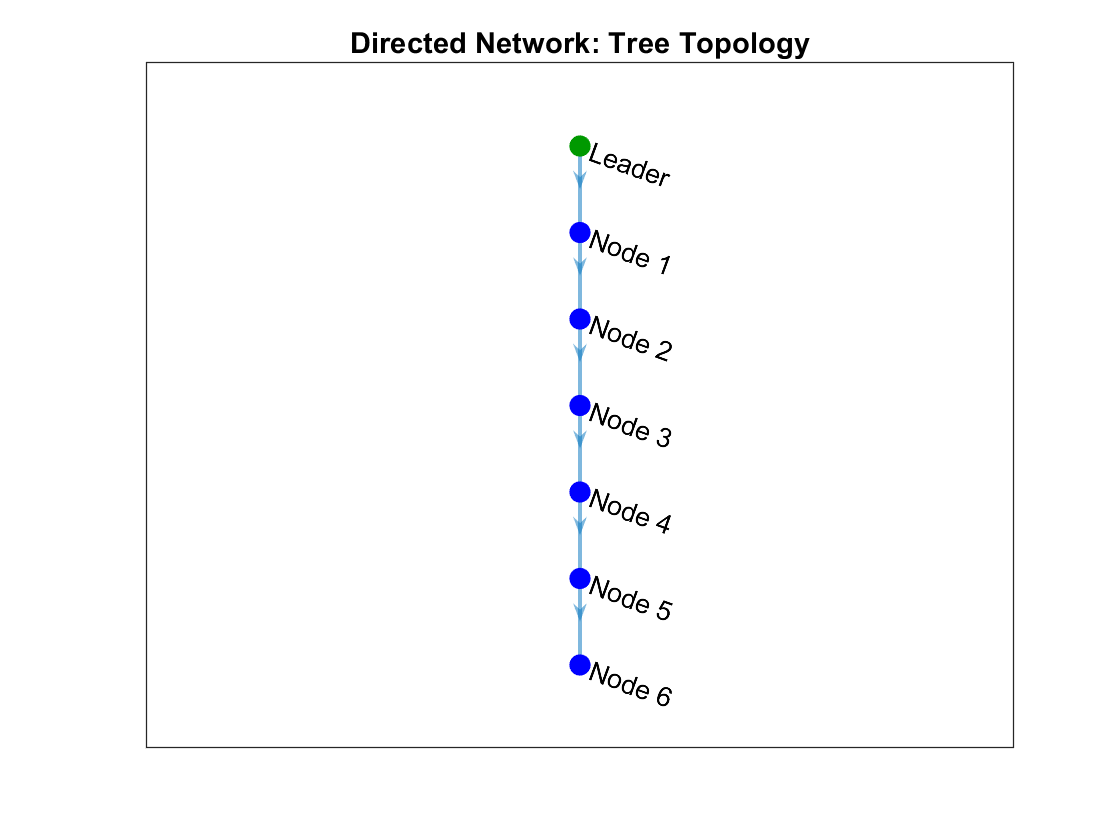
\includegraphics[width=0.50\textwidth]{tree_topology_graph.png} % Adjust width as needed
    \caption{The graph of the communication link in tree topology.}
\end{figure}

\subsection{Distributed control protocol with the local observer}
\subsubsection{Step reference}
\begin{figure}[H] % h means "here", can also use t (top), b (bottom), p (page)
    \centering
    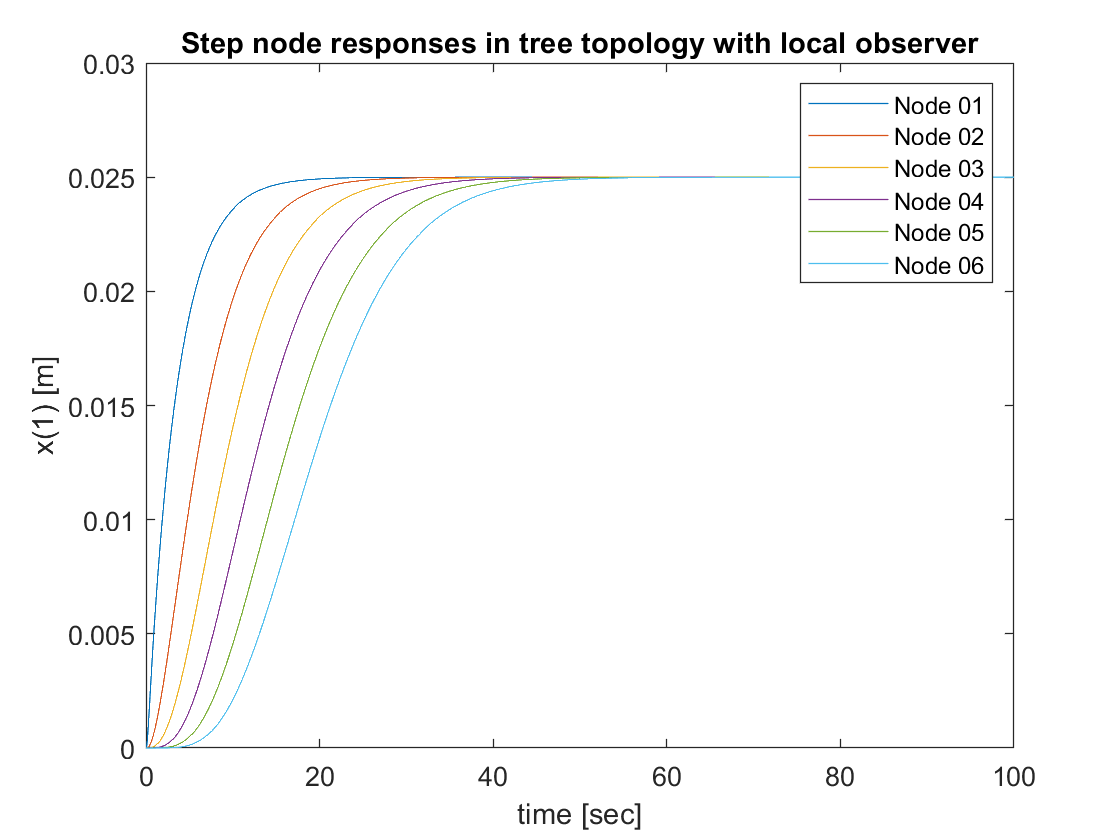
\includegraphics[width=0.50\textwidth]{step_tree_local.png} % Adjust width as needed
    \caption{The response of the nodes with the step reference in tree topology by local observer.}
\end{figure}

\subsubsection{Ramp reference}
\begin{figure}[H] % h means "here", can also use t (top), b (bottom), p (page)
    \centering
    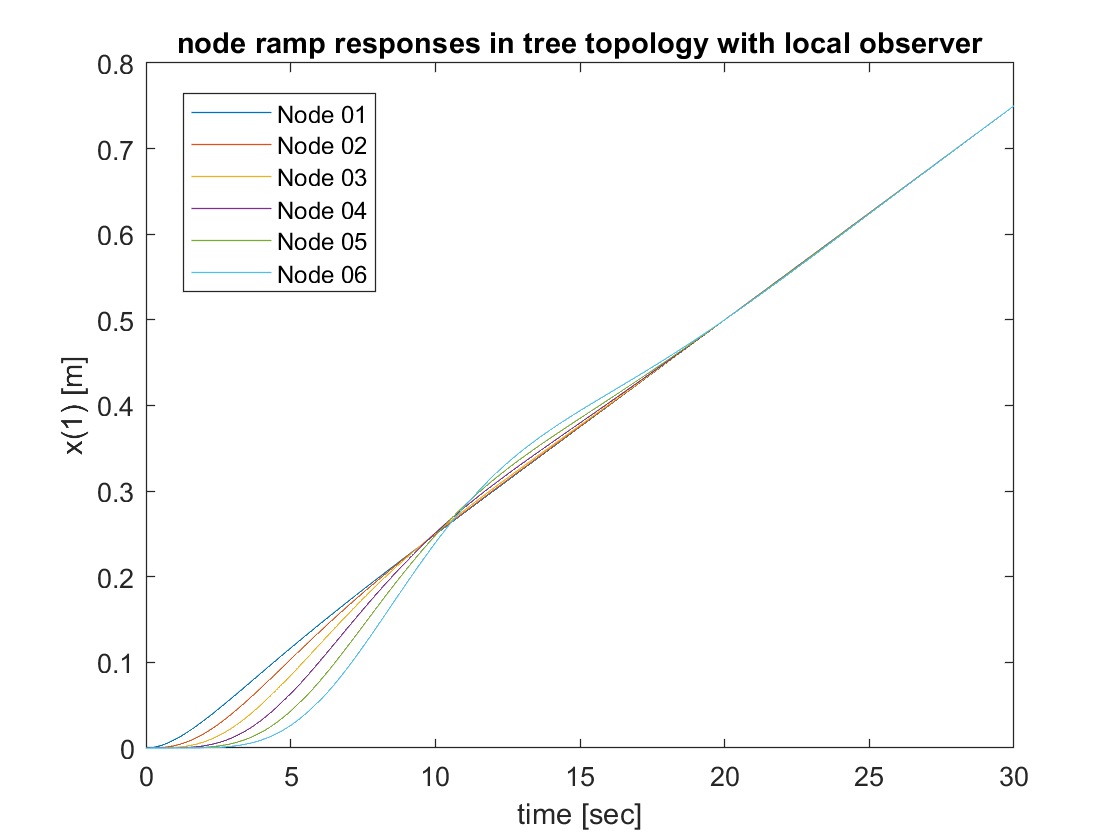
\includegraphics[width=0.50\textwidth]{ramp_tree_local.png} % Adjust width as needed
    \caption{The response of the nodes with the ramp reference in tree topology by local observer.}
\end{figure}


\subsubsection{Sinusoidal reference}
\begin{figure}[H] % h means "here", can also use t (top), b (bottom), p (page)
    \centering
    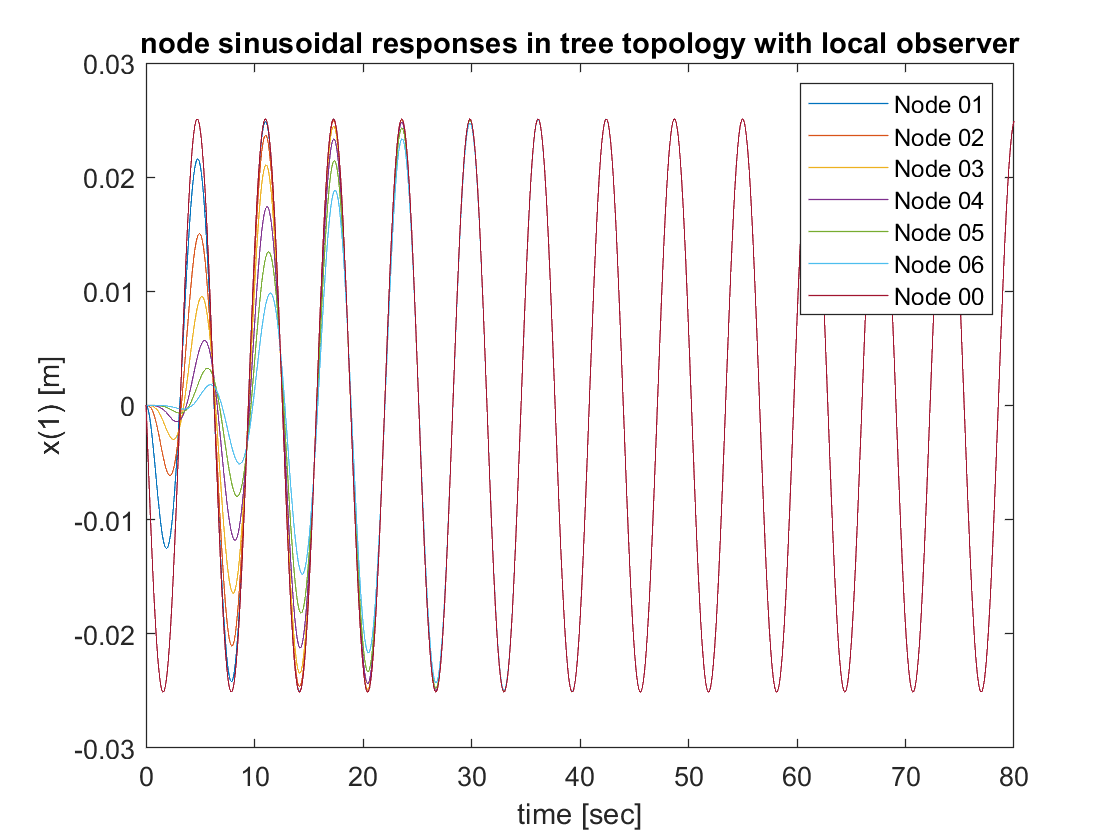
\includegraphics[width=0.50\textwidth]{sin_tree_local.png} % Adjust width as needed
    \caption{The response of the nodes with the sin reference in tree topology by local observer.}
\end{figure}



\subsection{Distributed control protocol with the global observer}
\subsubsection{Step reference}
\begin{figure}[H] % h means "here", can also use t (top), b (bottom), p (page)
    \centering
    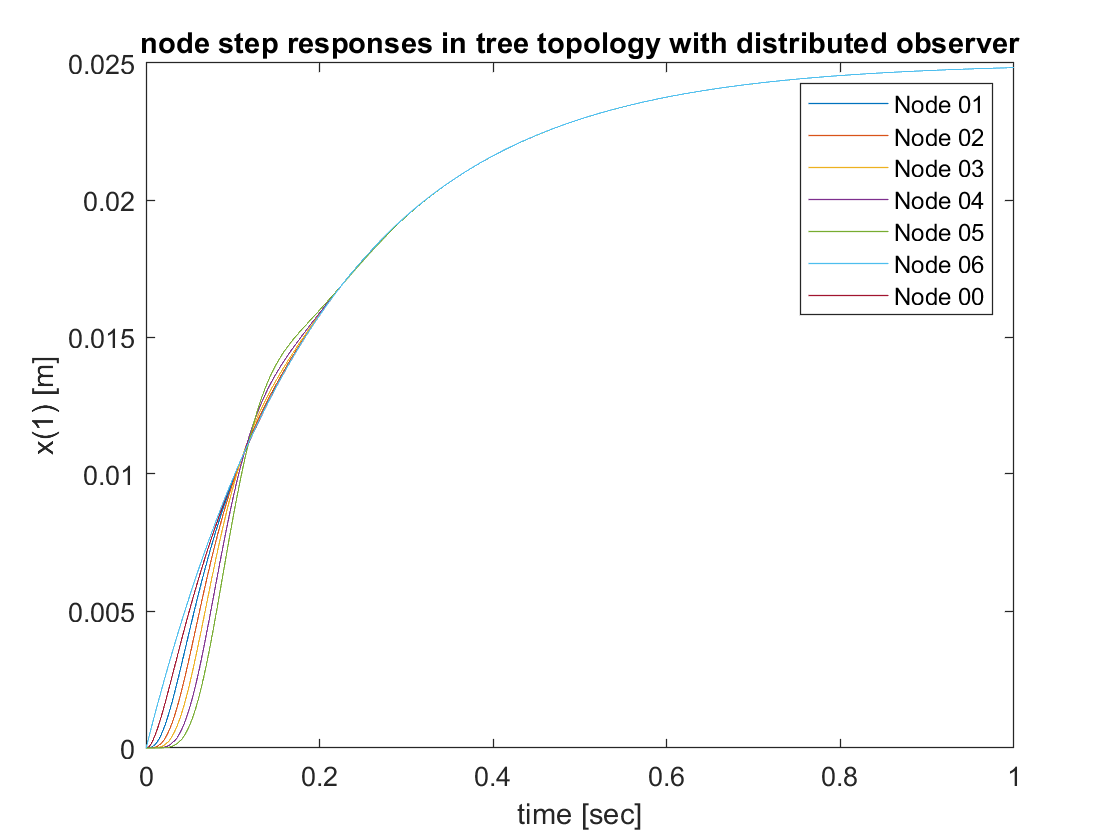
\includegraphics[width=0.50\textwidth]{step_tree_distributed.png} % Adjust width as needed
    \caption{The response of the nodes with the step reference in tree topology by global observer.}
\end{figure}

\subsubsection{Ramp reference}
\begin{figure}[H] % h means "here", can also use t (top), b (bottom), p (page)
    \centering
    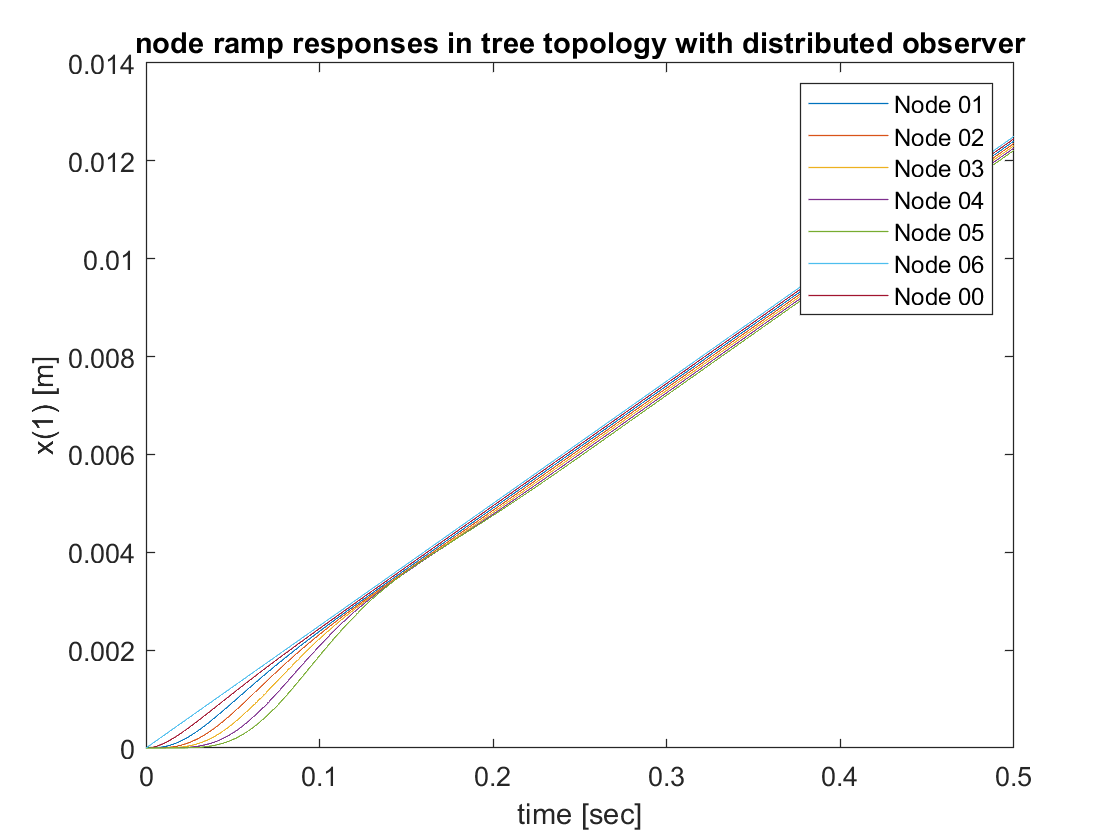
\includegraphics[width=0.50\textwidth]{ramp_tree_distributed.png} % Adjust width as needed
    \caption{The response of the nodes with the ramp reference in tree topology by global observer.}
\end{figure}


\subsubsection{Sinusoidal reference}
\begin{figure}[H] % h means "here", can also use t (top), b (bottom), p (page)
    \centering
    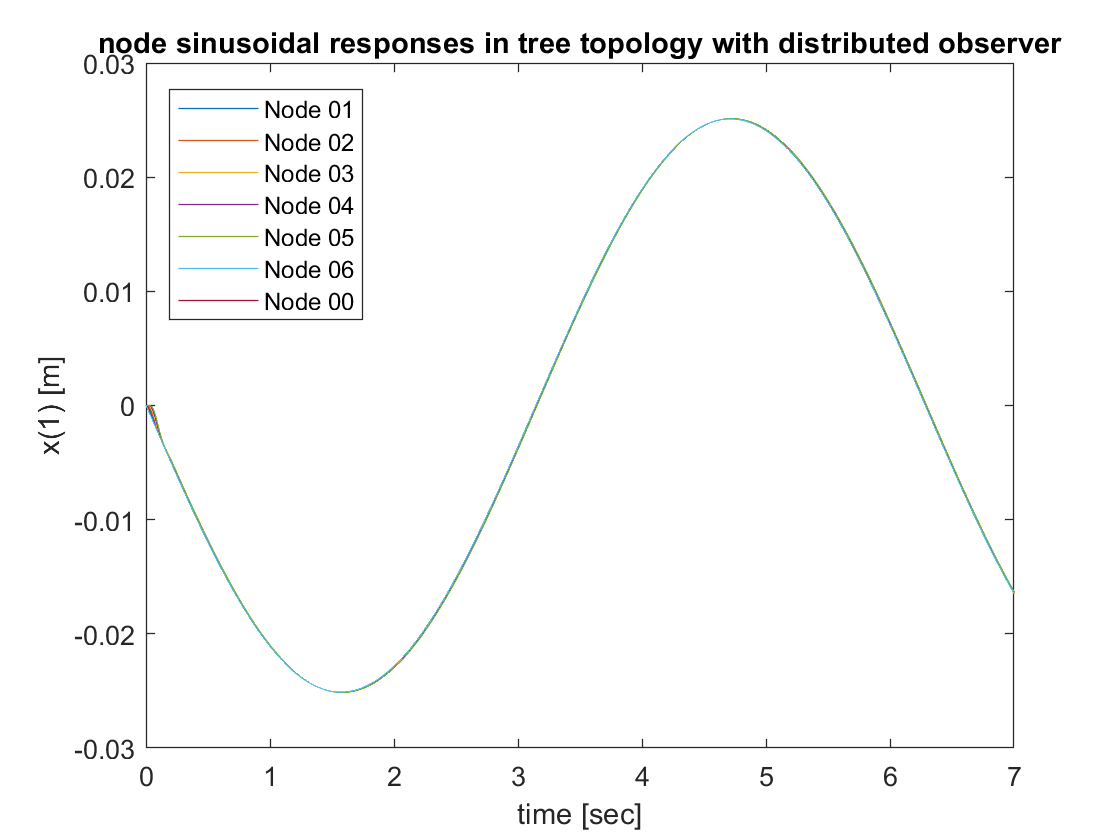
\includegraphics[width=0.50\textwidth]{sin_tree_distributed.png} % Adjust width as needed
    \caption{The response of the nodes with the sin reference in tree topology by global observer.}
\end{figure}


%%%%%%%%%%%%%%%%%%%%%%%%%%%%
%%%%%%%%%%%%%%%%%%%%%%%%%%%%
%%%%%%%%%%%%%%%%%%%%%%%%%%%%
%%%%%%%%%%%%%%%%%%%%%%%%%%%%
\subsection{Investigating Ring Topology}
The graph of this topology is as follows:
\begin{figure}[H] % h means "here", can also use t (top), b (bottom), p (page)
    \centering
    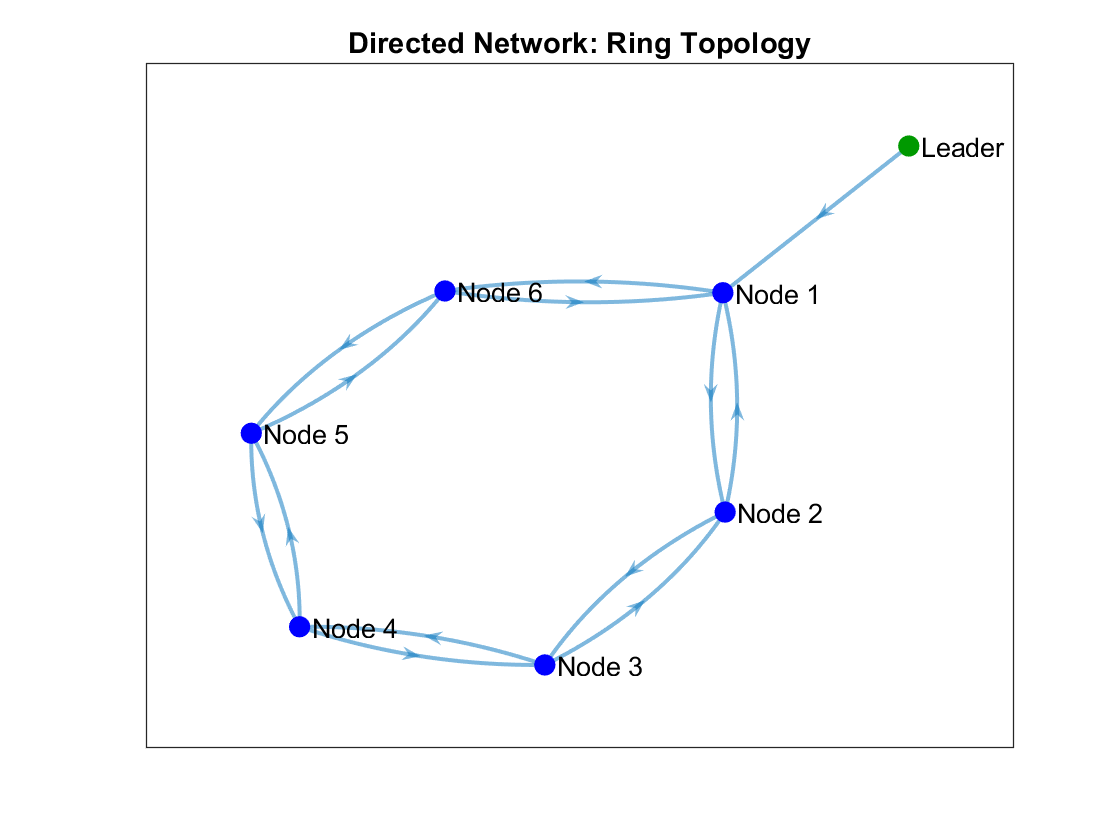
\includegraphics[width=0.55\textwidth]{ring_topology_graph.png} % Adjust width as needed
    \caption{The graph of the communication link in ring topology.}
\end{figure}

\subsection{Distributed control protocol with the local observer}
\subsubsection{Step reference}
\begin{figure}[H] % h means "here", can also use t (top), b (bottom), p (page)
    \centering
    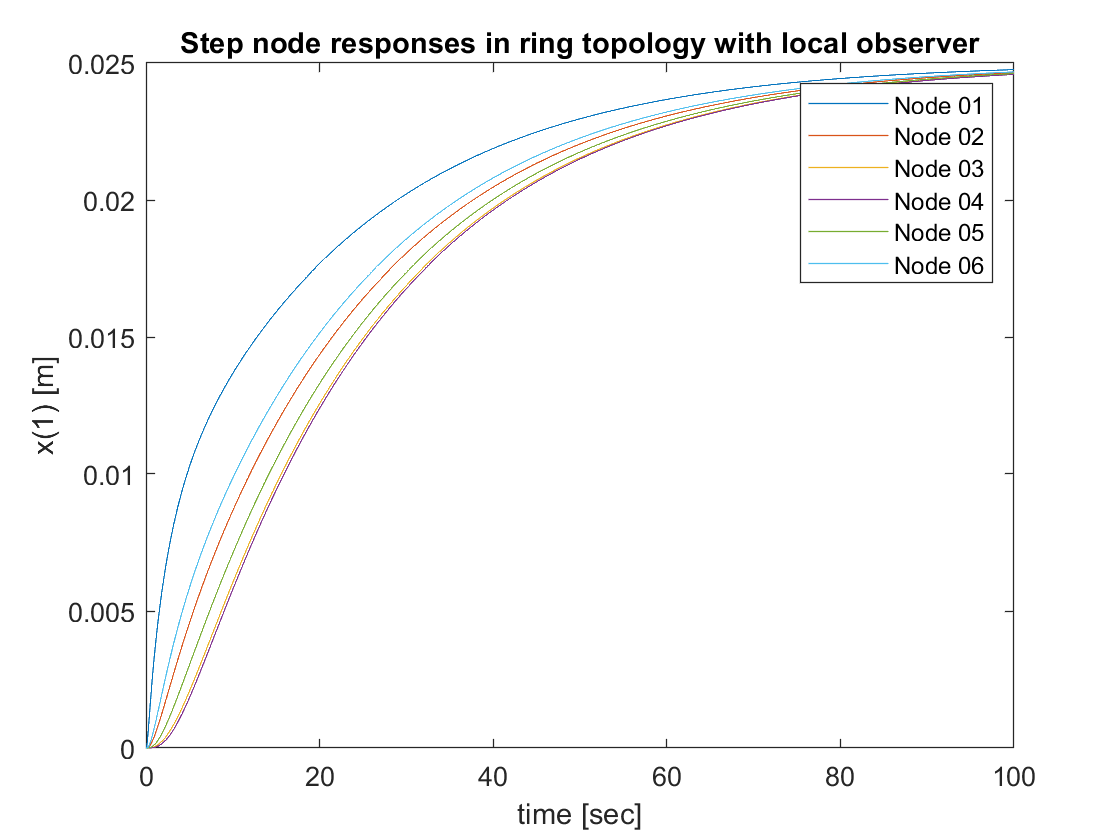
\includegraphics[width=0.50\textwidth]{step_ring_local.png} % Adjust width as needed
    \caption{The response of the nodes with the step reference in ring topology by local observer.}
\end{figure}

\subsubsection{Ramp reference}
\begin{figure}[H] % h means "here", can also use t (top), b (bottom), p (page)
    \centering
    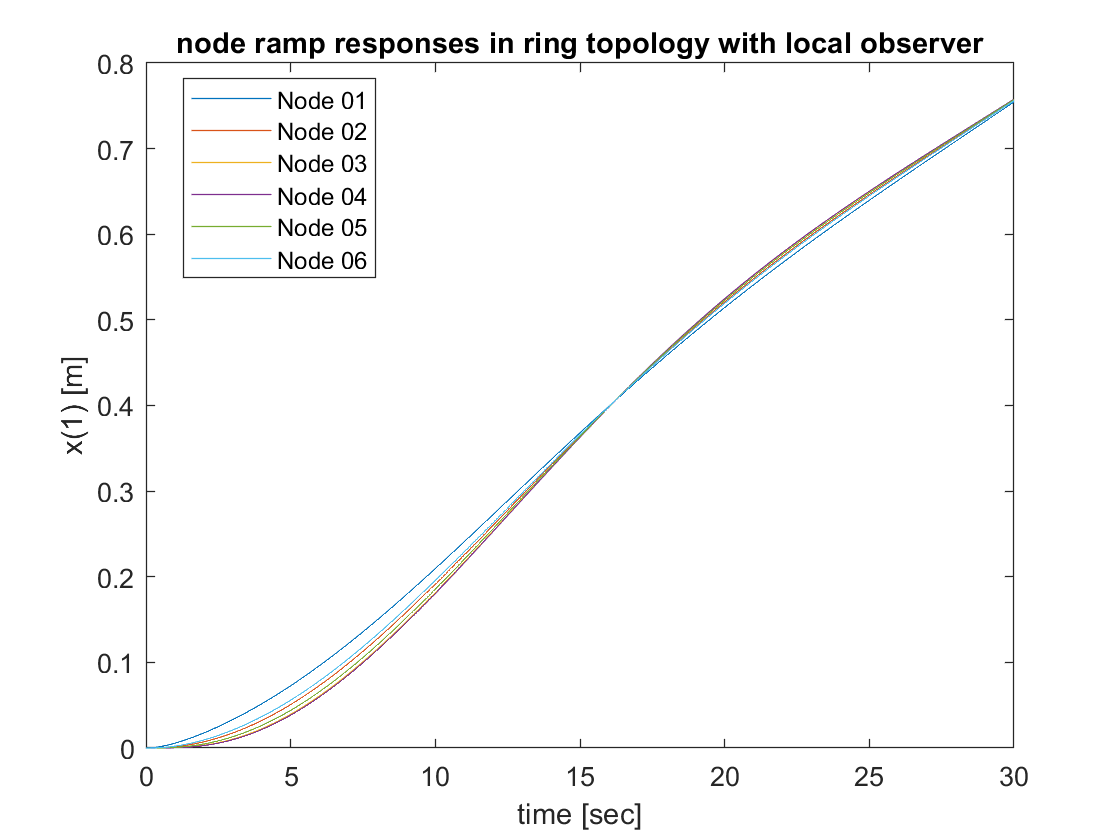
\includegraphics[width=0.50\textwidth]{ramp_ring_local.png} % Adjust width as needed
    \caption{The response of the nodes with the ramp reference in ring topology by local observer.}
\end{figure}

\subsubsection{Sinusoidal reference}
\begin{figure}[H] % h means "here", can also use t (top), b (bottom), p (page)
    \centering
    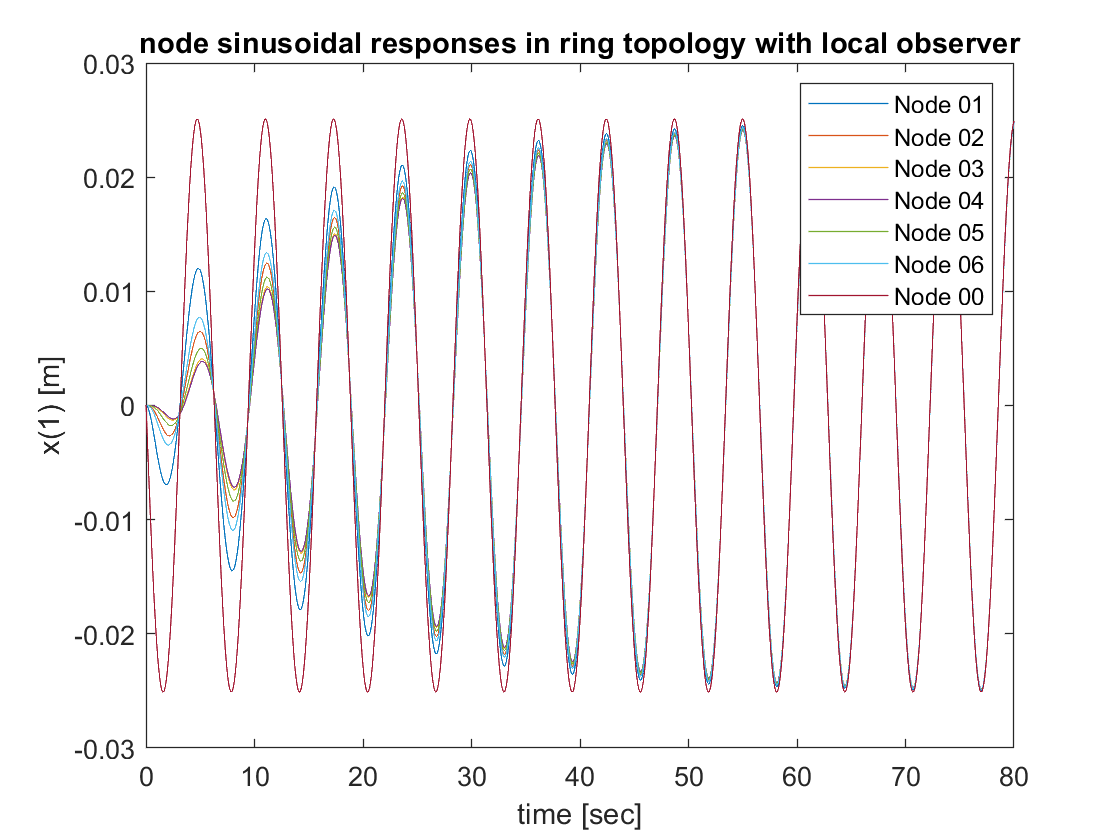
\includegraphics[width=0.50\textwidth]{sin_ring_local.png} % Adjust width as needed
    \caption{The response of the nodes with the sinusoidal reference in ring topology by local observer.}
\end{figure}



\subsection{Distributed control protocol with the global observer}
\subsubsection{Step reference}
\begin{figure}[H] % h means "here", can also use t (top), b (bottom), p (page)
    \centering
    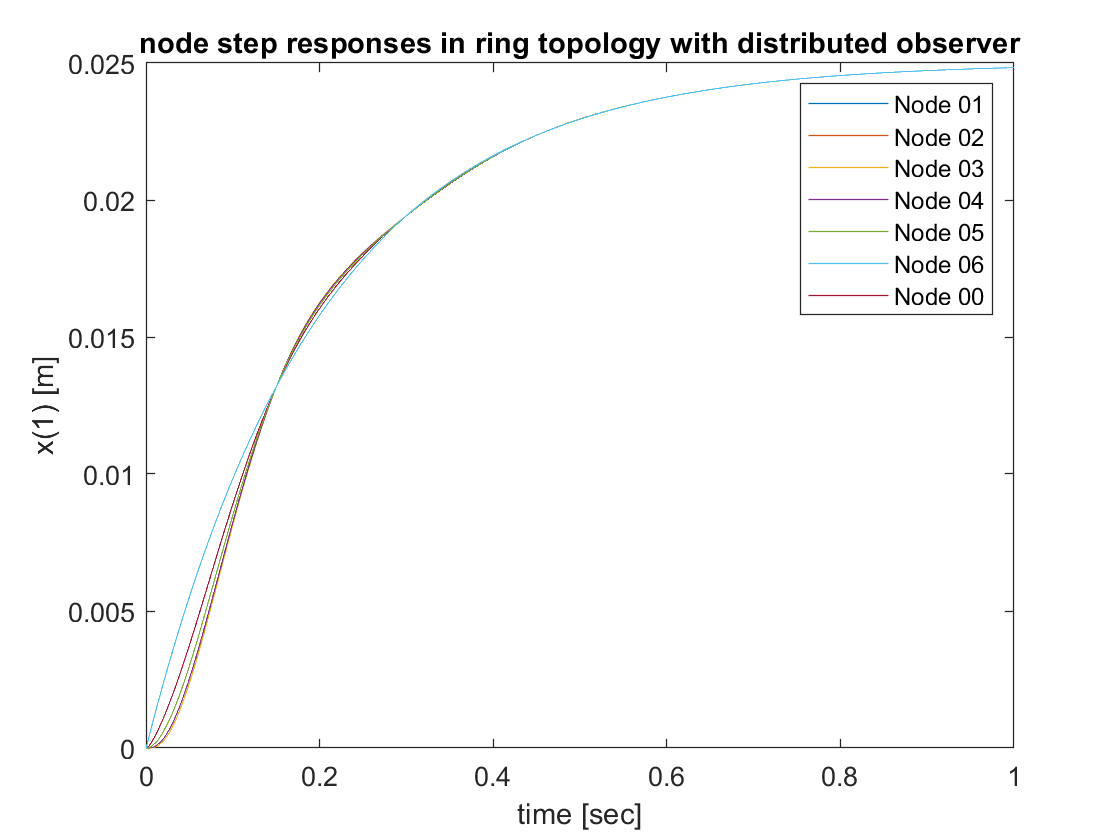
\includegraphics[width=0.50\textwidth]{step_ring_distributed.png} % Adjust width as needed
    \caption{The response of the nodes with the step reference in ring topology by global observer.}
\end{figure}

\subsubsection{Ramp reference}
\begin{figure}[H] % h means "here", can also use t (top), b (bottom), p (page)
    \centering
    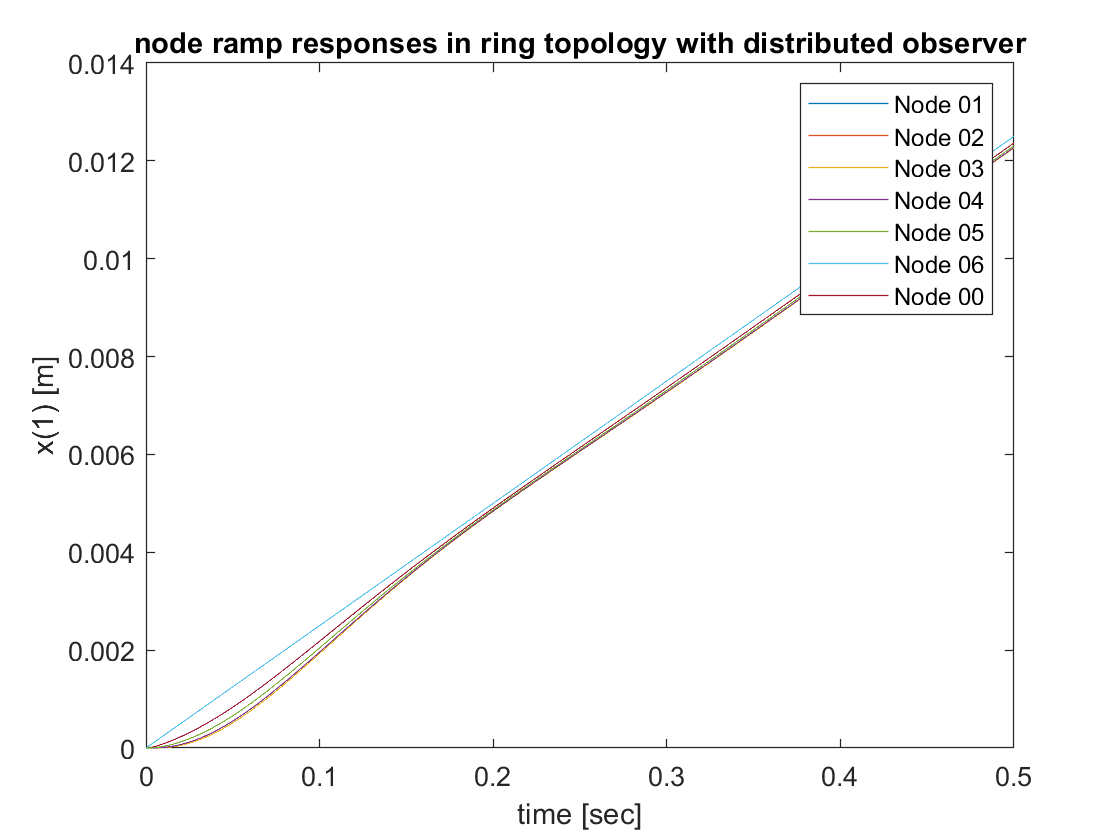
\includegraphics[width=0.50\textwidth]{ramp_ring_distributed.png} % Adjust width as needed
    \caption{The response of the nodes with the ramp reference in ring topology by global observer.}
\end{figure}

\subsubsection{Sinusoidal reference}
\begin{figure}[H] % h means "here", can also use t (top), b (bottom), p (page)
    \centering
    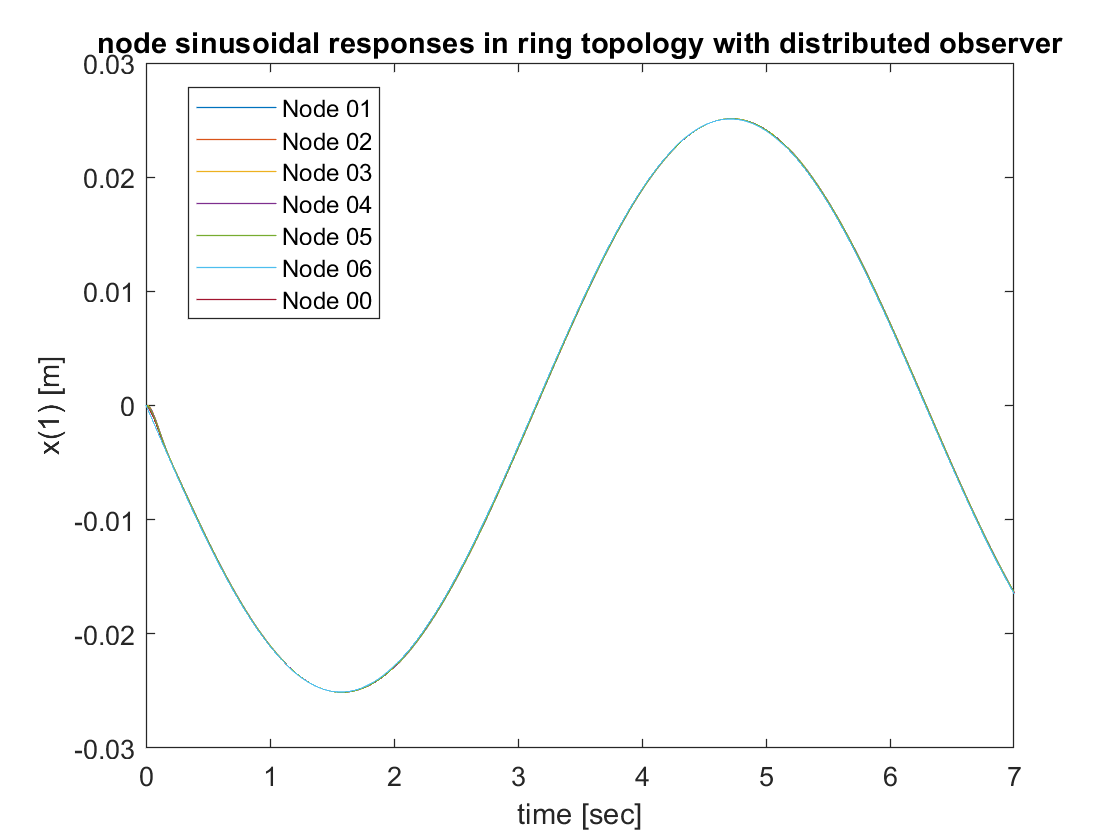
\includegraphics[width=0.50\textwidth]{sin_ring_distributed.png} % Adjust width as needed
    \caption{The response of the nodes with the sinusoidal reference in ring topology by global observer.}
\end{figure}

%%%%%%%%%%%%%%%%%%%%%%%%%%%%
%%%%%%%%%%%%%%%%%%%%%%%%%%%%
%%%%%%%%%%%%%%%%%%%%%%%%%%%%
%%%%%%%%%%%%%%%%%%%%%%%%%%%%
\subsection{Investigating fully connected Topology}
The graph of this topology is as follows:
\begin{figure}[H] % h means "here", can also use t (top), b (bottom), p (page)
    \centering
    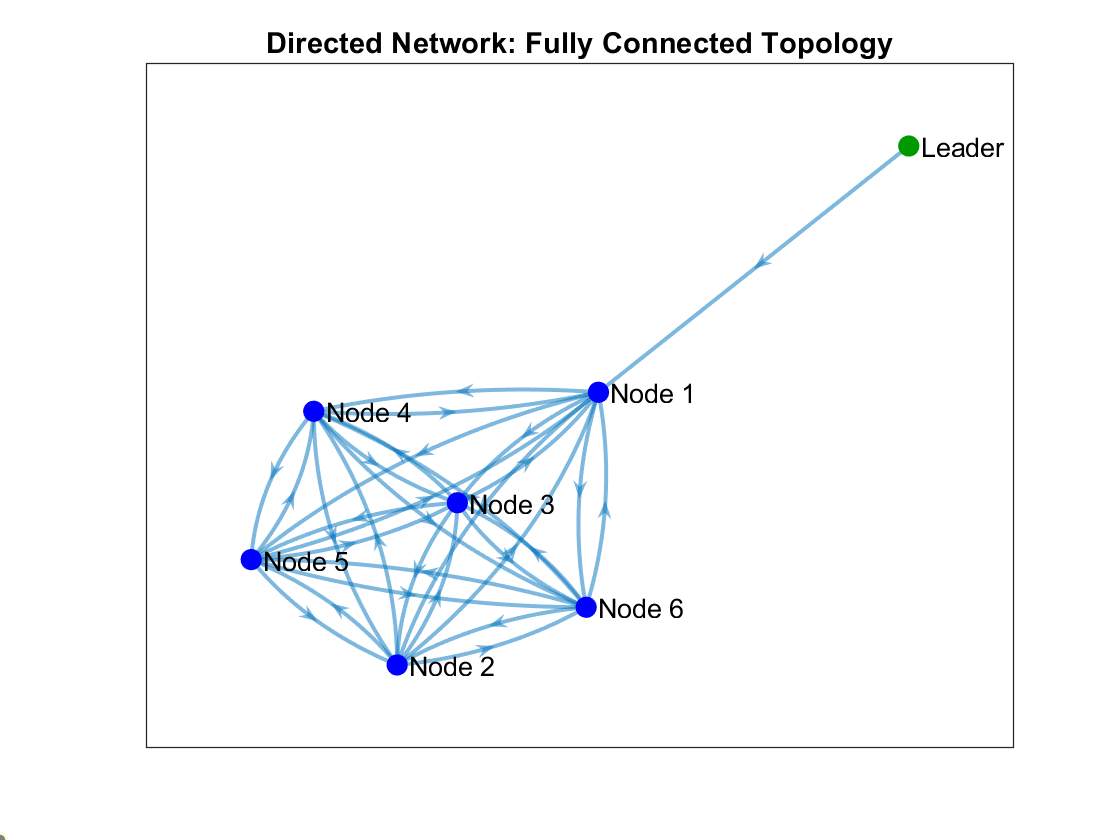
\includegraphics[width=0.55\textwidth]{full_topology_graph.png} % Adjust width as needed
    \caption{The graph of the communication link in fully connected topology.}
\end{figure}

\subsection{Distributed control protocol with the local observer}
\subsubsection{Step reference}
\begin{figure}[H] % h means "here", can also use t (top), b (bottom), p (page)
    \centering
    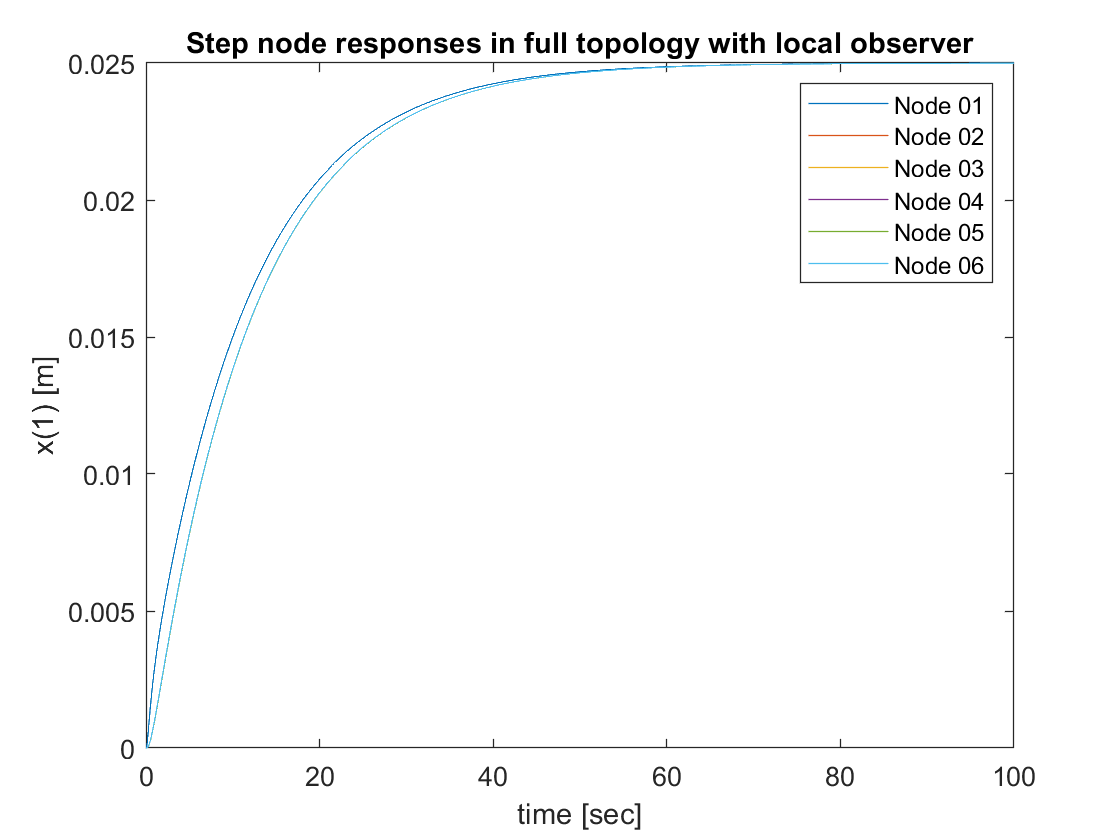
\includegraphics[width=0.50\textwidth]{step_full_local.png} % Adjust width as needed
    \caption{The response of the nodes with the step reference in fully connected topology by local observer.}
\end{figure}


\subsubsection{Ramp reference}
\begin{figure}[H] % h means "here", can also use t (top), b (bottom), p (page)
    \centering
    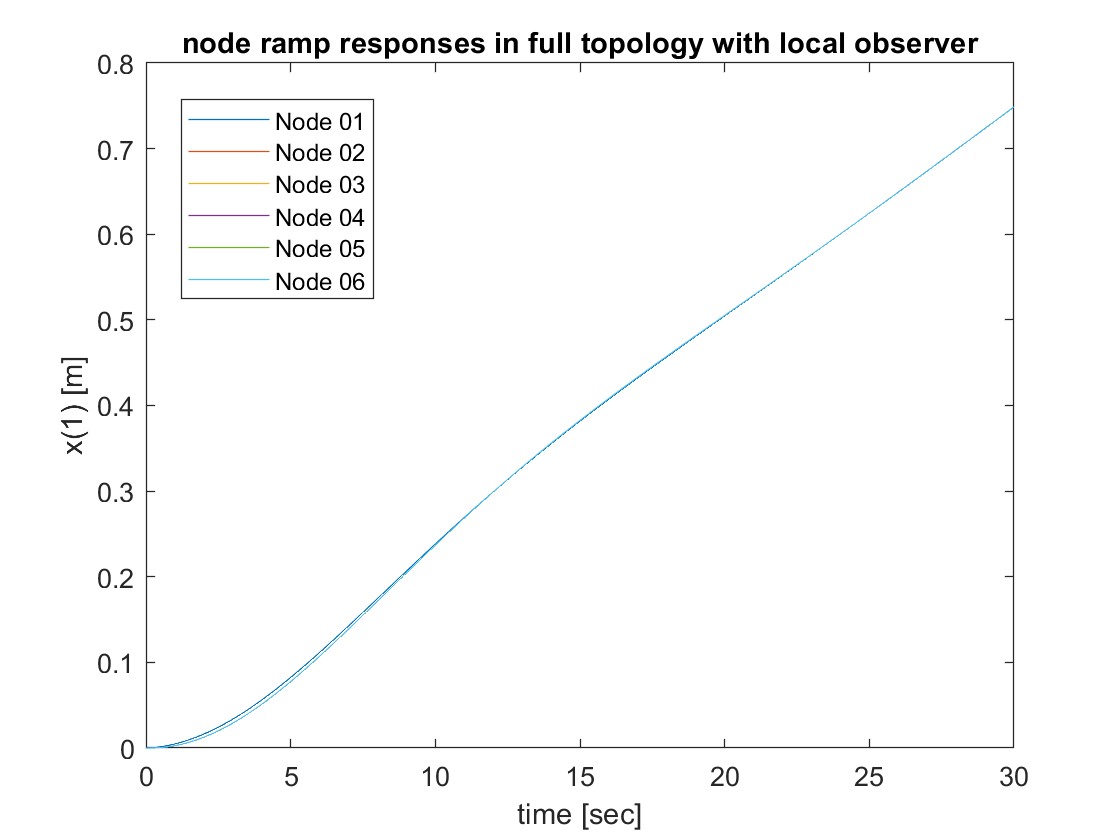
\includegraphics[width=0.50\textwidth]{ramp_full_local.png} % Adjust width as needed
    \caption{The response of the nodes with the ramp reference in fully connected topology by local observer.}
\end{figure}

\subsubsection{Sinusoidal reference}
\begin{figure}[H] % h means "here", can also use t (top), b (bottom), p (page)
    \centering
    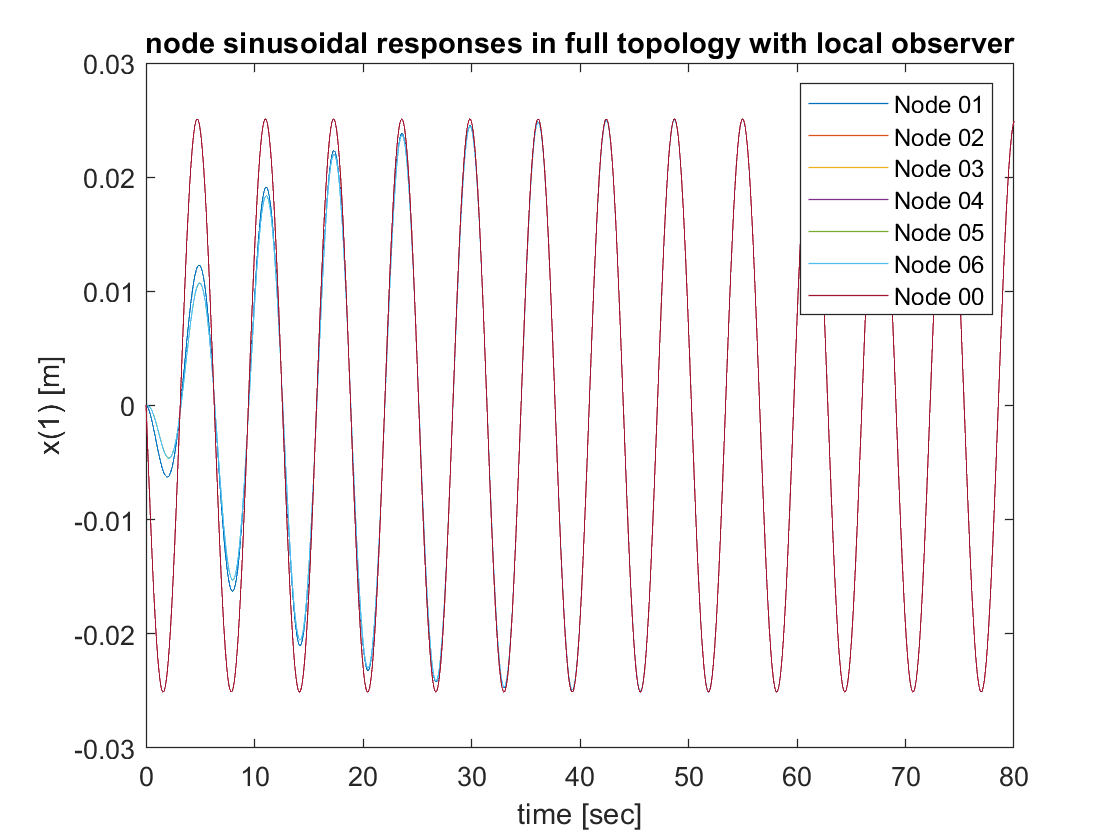
\includegraphics[width=0.50\textwidth]{sin_full_local.png} % Adjust width as needed
    \caption{The response of the nodes with the sinusoidal reference in fully connected topology by local observer.}
\end{figure}

\subsection{Distributed control protocol with the global observer}
\subsubsection{Step reference}
\begin{figure}[H] % h means "here", can also use t (top), b (bottom), p (page)
    \centering
    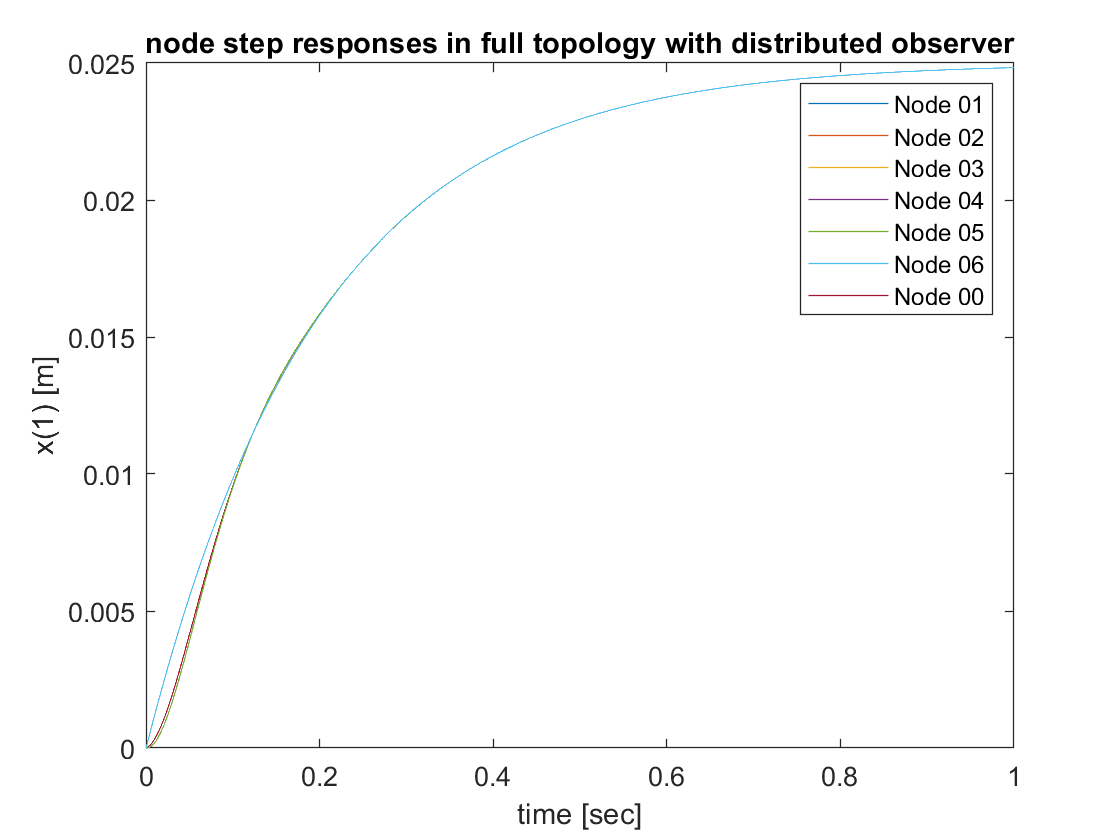
\includegraphics[width=0.50\textwidth]{step_full_distributed.png} % Adjust width as needed
    \caption{The response of the nodes with the step reference in fully connected topology by global observer.}
\end{figure}


\subsubsection{Ramp reference}
\begin{figure}[H] % h means "here", can also use t (top), b (bottom), p (page)
    \centering
    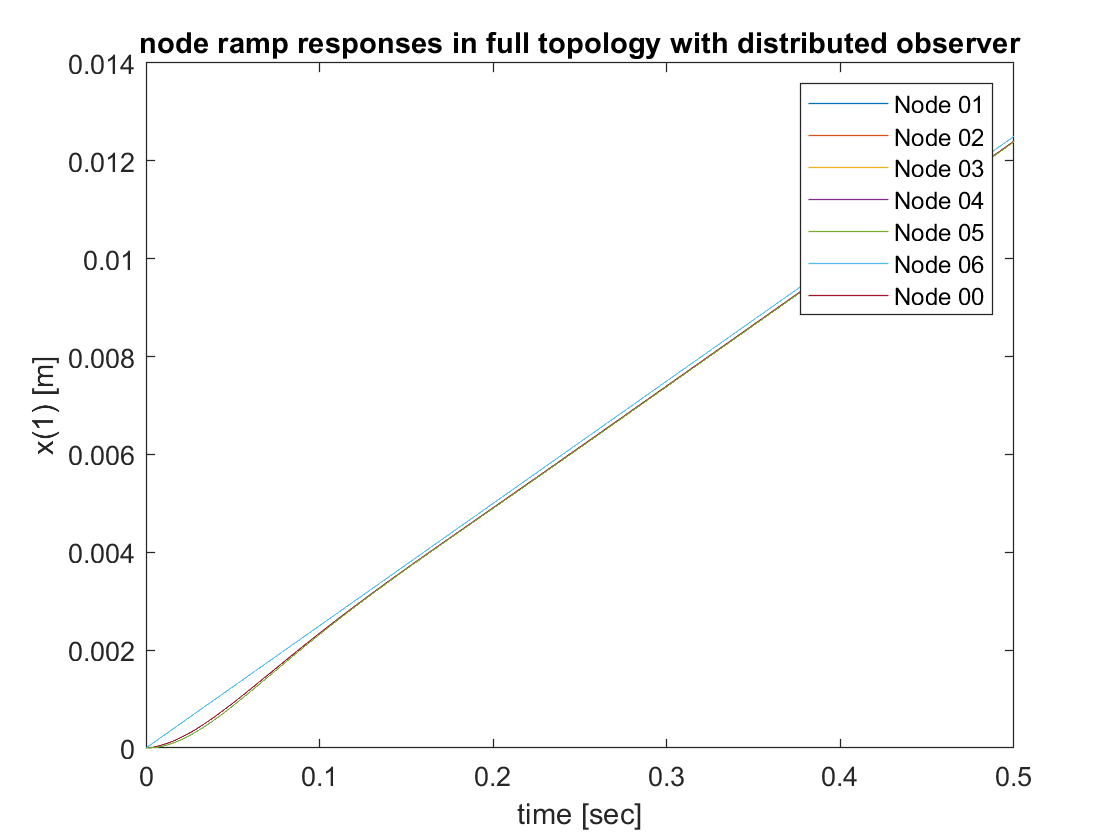
\includegraphics[width=0.50\textwidth]{ramp_full_distributed.png} % Adjust width as needed
    \caption{The response of the nodes with the ramp reference in fully connected topology by global observer.}
\end{figure}

\subsubsection{Sinusoidal reference}
\begin{figure}[H] % h means "here", can also use t (top), b (bottom), p (page)
    \centering
    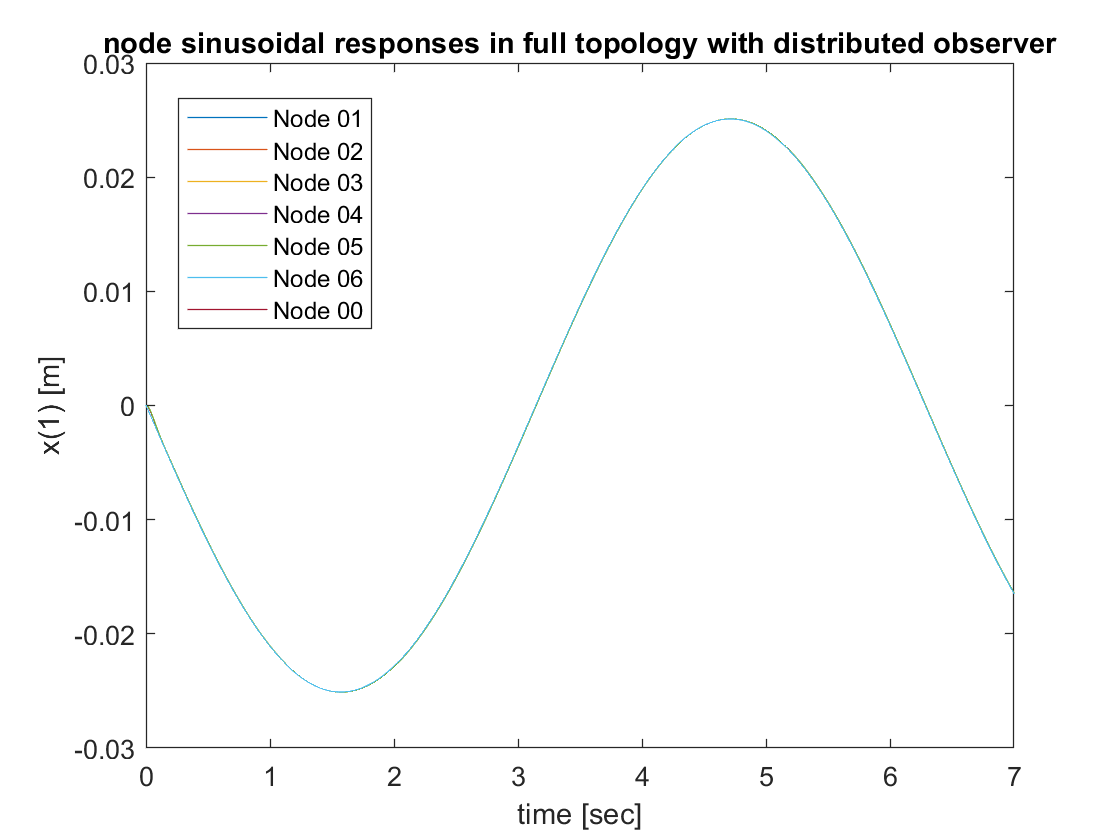
\includegraphics[width=0.50\textwidth]{sin_full_distributed.png} % Adjust width as needed
    \caption{The response of the nodes with the sinusoidal reference in fully connected topology by global observer.}
\end{figure}


%%%%%%%%%%%%%%%%%%%%%%%%%%%%
%%%%%%%%%%%%%%%%%%%%%%%%%%%%
%%%%%%%%%%%%%%%%%%%%%%%%%%%%
%%%%%%%%%%%%%%%%%%%%%%%%%%%%
\subsection{Investigating star Topology}
The graph of this topology is as follows:
\begin{figure}[H] % h means "here", can also use t (top), b (bottom), p (page)
    \centering
    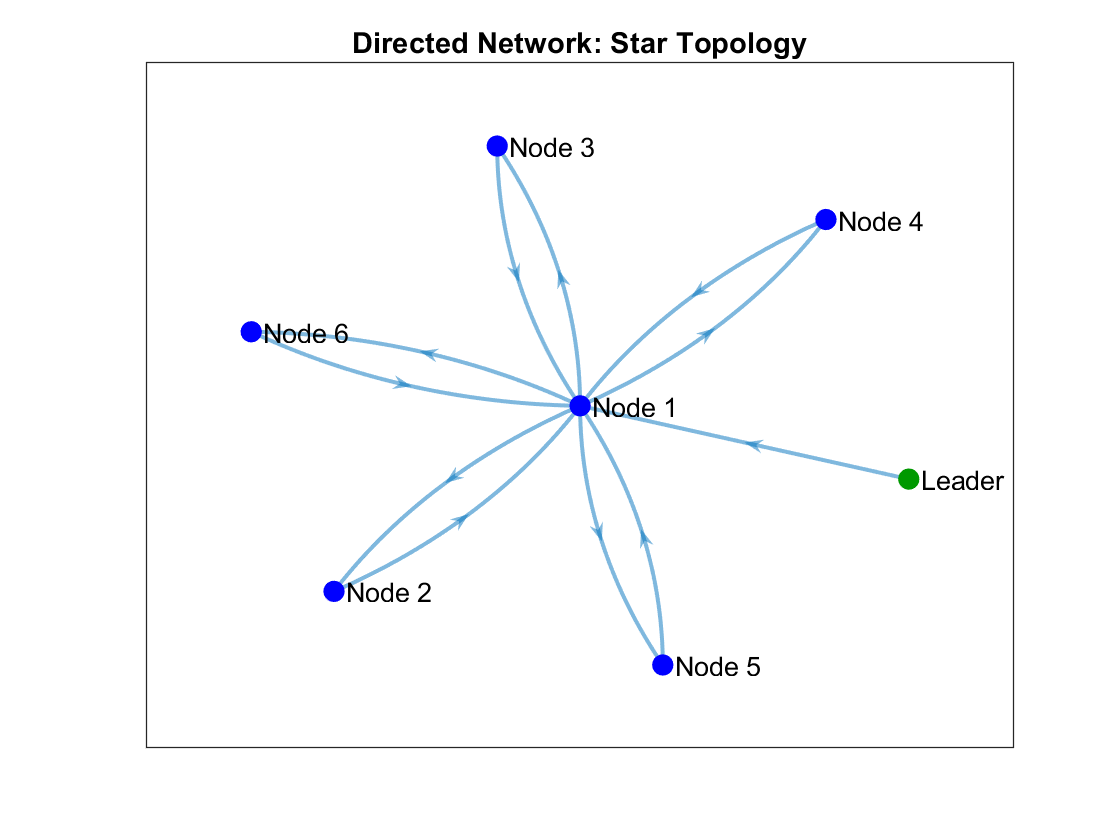
\includegraphics[width=0.75\textwidth]{star_topology_graph.png} % Adjust width as needed
    \caption{The graph of the communication link in star topology.}
\end{figure}

\subsection{Distributed control protocol with the local observer}
\subsubsection{Step reference}
\begin{figure}[H] % h means "here", can also use t (top), b (bottom), p (page)
    \centering
    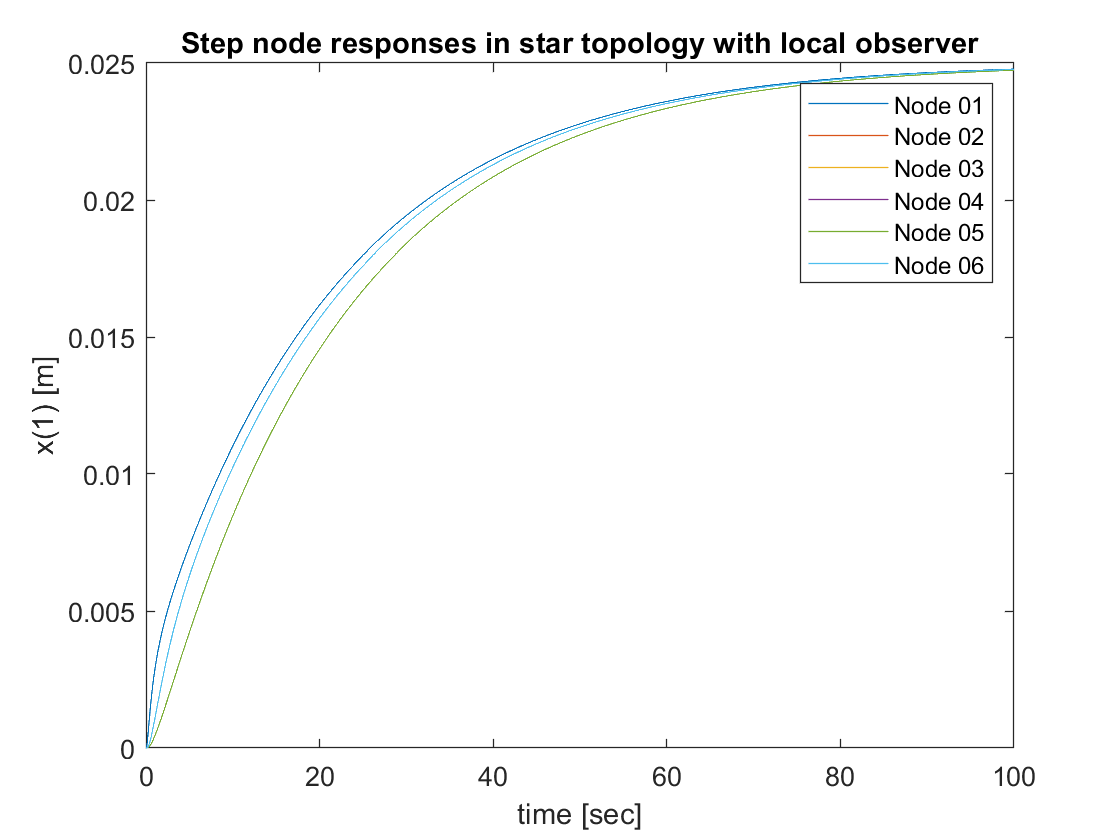
\includegraphics[width=0.50\textwidth]{step_star_local.png} % Adjust width as needed
    \caption{The response of the nodes with the step reference in star topology by local observer.}
\end{figure}
In this case, again it can be observed that the rising time is not as fast as the other nodes. It is true that  the lag among the nodes is not as small as fully connected network; nevertheless, the gap is not that much considerable with respect to tree and ring.

\subsubsection{Ramp reference}
\begin{figure}[H] % h means "here", can also use t (top), b (bottom), p (page)
    \centering
    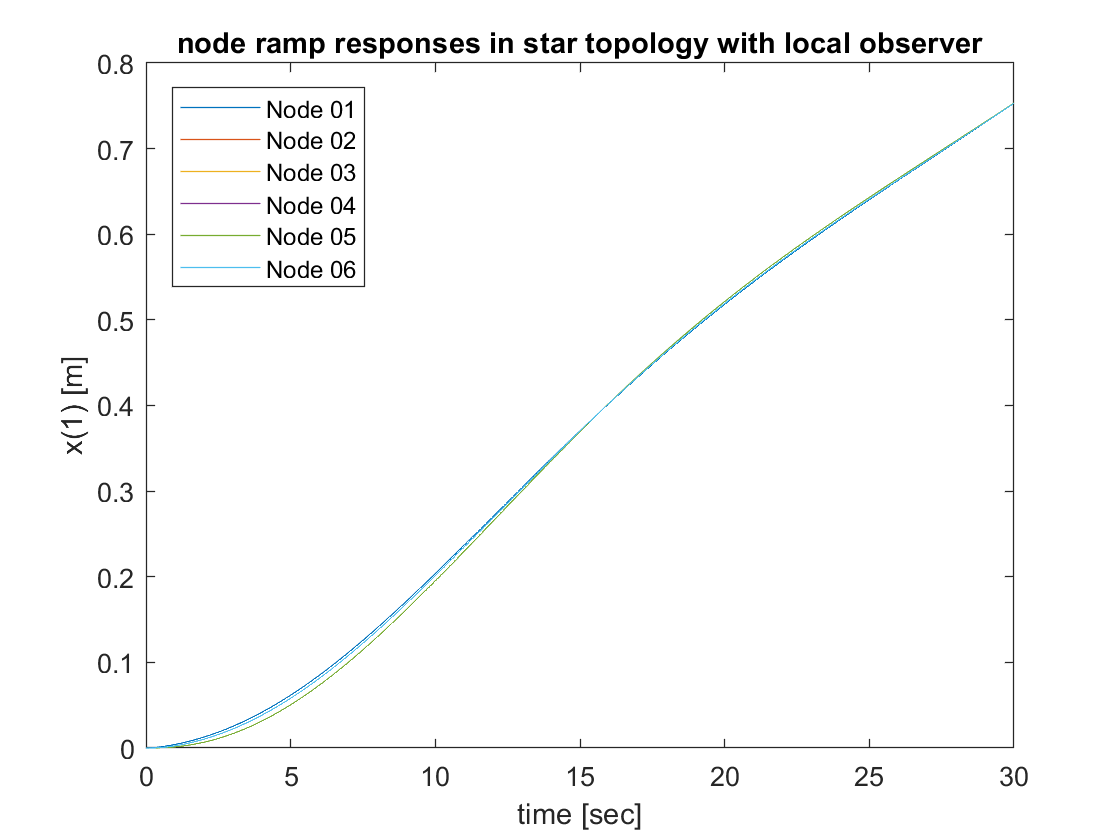
\includegraphics[width=0.50\textwidth]{ramp_star_local.png} % Adjust width as needed
    \caption{The response of the nodes with the ramp reference in star topology by local observer.}
\end{figure}

\subsubsection{Sinusoidal reference}
\begin{figure}[H] % h means "here", can also use t (top), b (bottom), p (page)
    \centering
    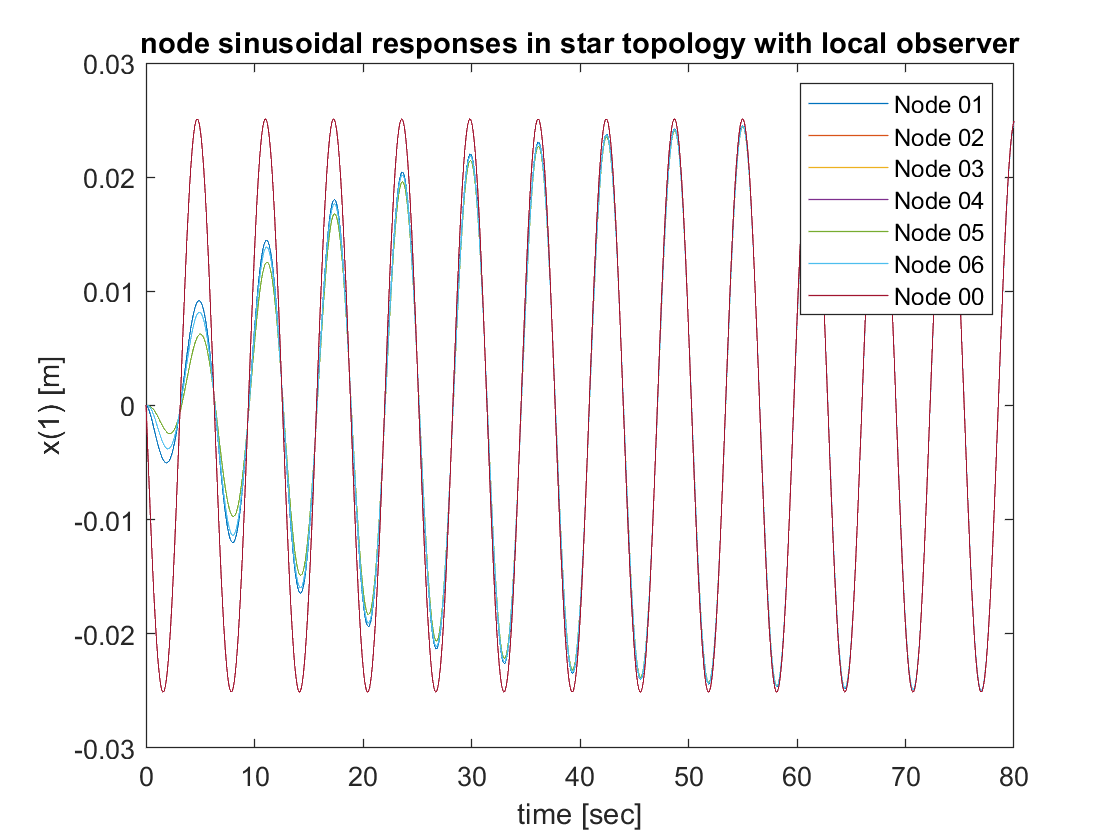
\includegraphics[width=0.50\textwidth]{sin_star_local.png} % Adjust width as needed
    \caption{The response of the nodes with the sinusoidal reference in star topology by local observer.}
\end{figure}

\subsection{Distributed control protocol with the global observer}
\subsubsection{Step reference}
\begin{figure}[H] % h means "here", can also use t (top), b (bottom), p (page)
    \centering
    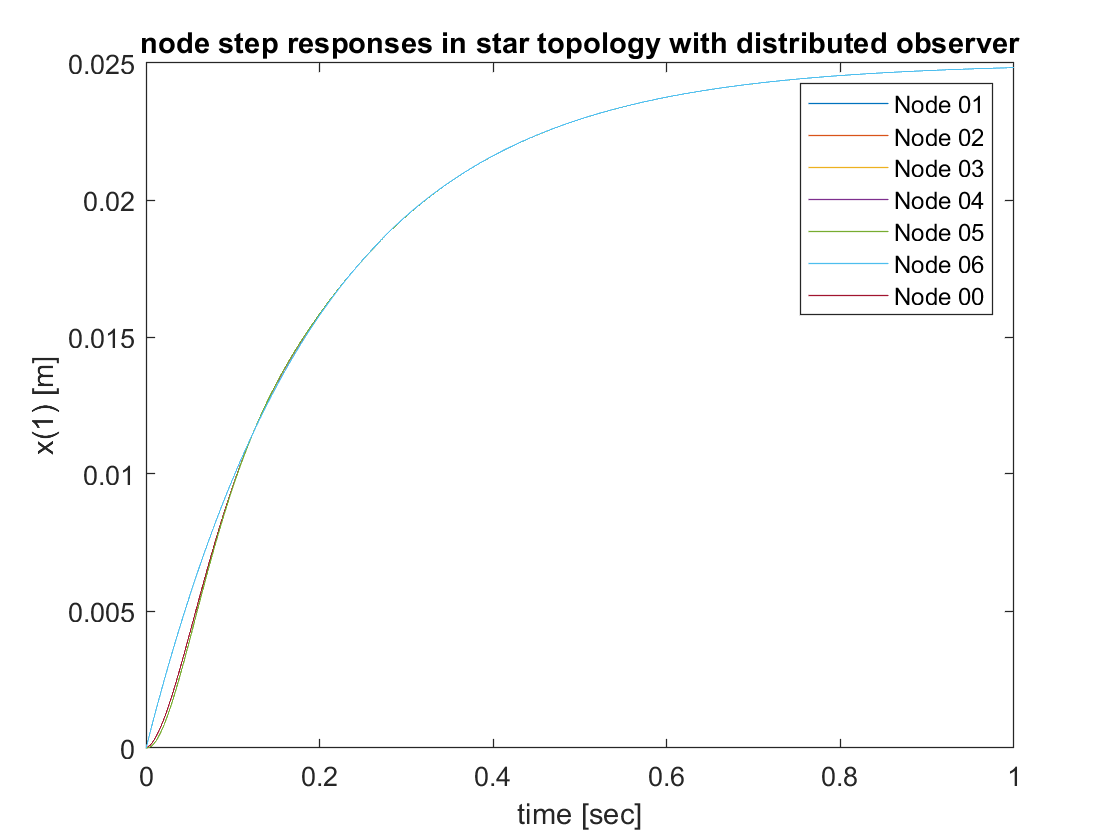
\includegraphics[width=0.50\textwidth]{step_star_distributed.png} % Adjust width as needed
    \caption{The response of the nodes with the step reference in star topology by global observer.}
\end{figure}
In this case, again it can be observed that the rising time is not as fast as the other nodes. It is true that  the lag among the nodes is not as small as fully connected network; nevertheless, the gap is not that much considerable with respect to tree and ring.

\subsubsection{Ramp reference}
\begin{figure}[H] % h means "here", can also use t (top), b (bottom), p (page)
    \centering
    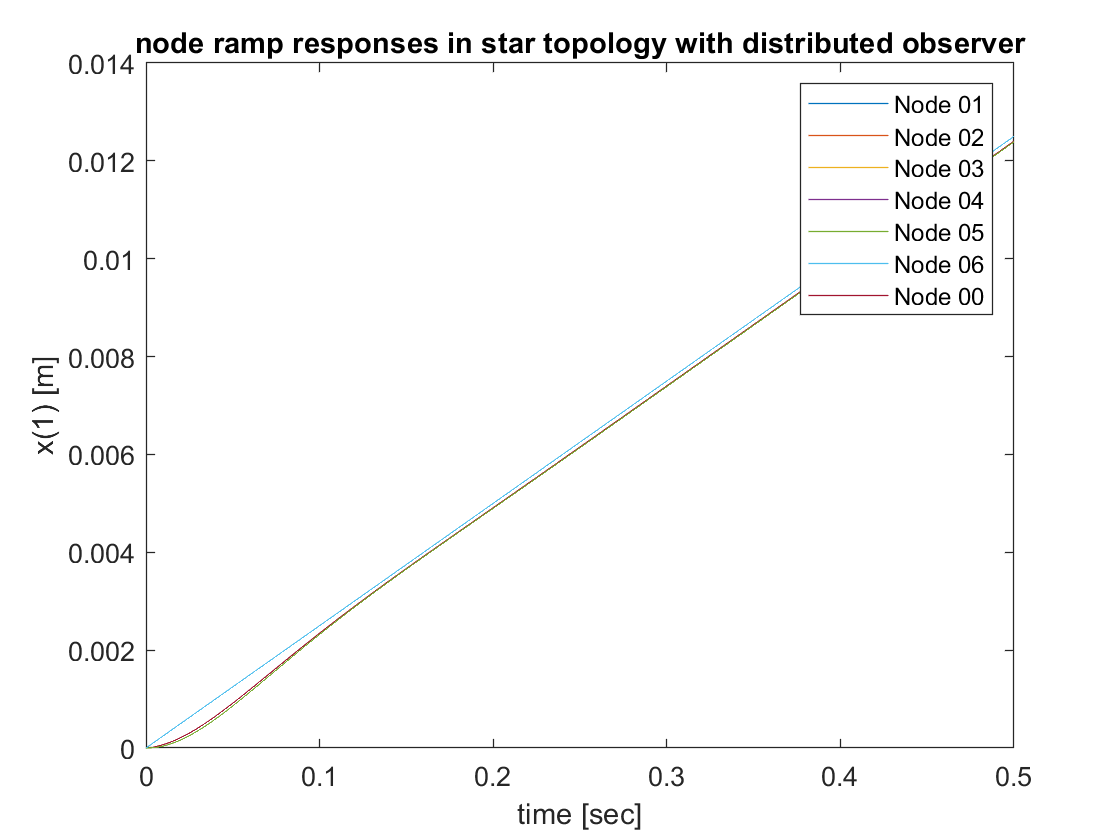
\includegraphics[width=0.50\textwidth]{ramp_star_distributed.png} % Adjust width as needed
    \caption{The response of the nodes with the ramp reference in star topology by global observer.}
\end{figure}

\subsubsection{Sinusoidal reference}
\begin{figure}[H] % h means "here", can also use t (top), b (bottom), p (page)
    \centering
    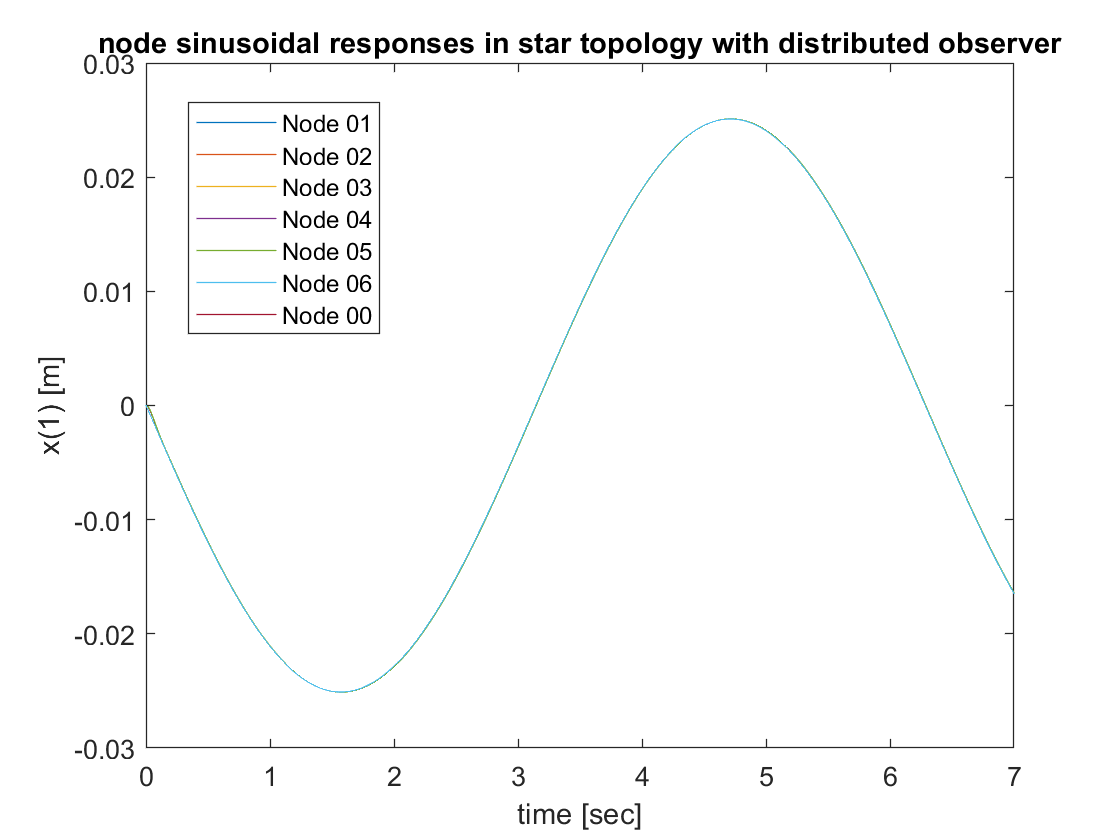
\includegraphics[width=0.50\textwidth]{sin_star_distributed.png} % Adjust width as needed
    \caption{The response of the nodes with the sinusoidal reference in star topology by global observer.}
\end{figure}

\subsection{Comparing the performance of the difference topologies}
Regarding the performance, it can be seen that the fully connected graph, outperforms other topologies regardless of the reference to be track; nonetheless, in practice this structure includes a lot of communications, and thereby the change of packet loss increases. All in all, taking into account practical considerations and the performance, it can be observed that star topology shows a remarkable performance. Further, in practice a round-robin algorithm can be implemented for the communication of thet nodes with the center node.

\subsection{Comparing the performance of the local observer vs. global observer}
It can be seen that global observer has a really good performance, and in the case that a global observer is used a considerablly faster convergence time is obtained. Therefore, at least in simulation, without any doubt, the global observer outperform the local observer. However, as it can be seen in the following section, the discrete-time version of global observer does not have a satisfying performance.



\section{discretized implementation global observer}
Although in the continuous simulation global observers performs really well, it can be seen that in the discretized implementation of this version, the realize time performance does not show a really suitable transient behavior. Further this performance deteriorates as the sampling time decreases. Another observation is that, in the discrete-time version, the sampling time should match the coupling gain; the larger the coupling gain, the smaller should be sampling time.

The performance of the discrete-time global observer with different sampling times can be seen hereunder.
\begin{figure}[H] % h means "here", can also use t (top), b (bottom), p (page)
    \centering
    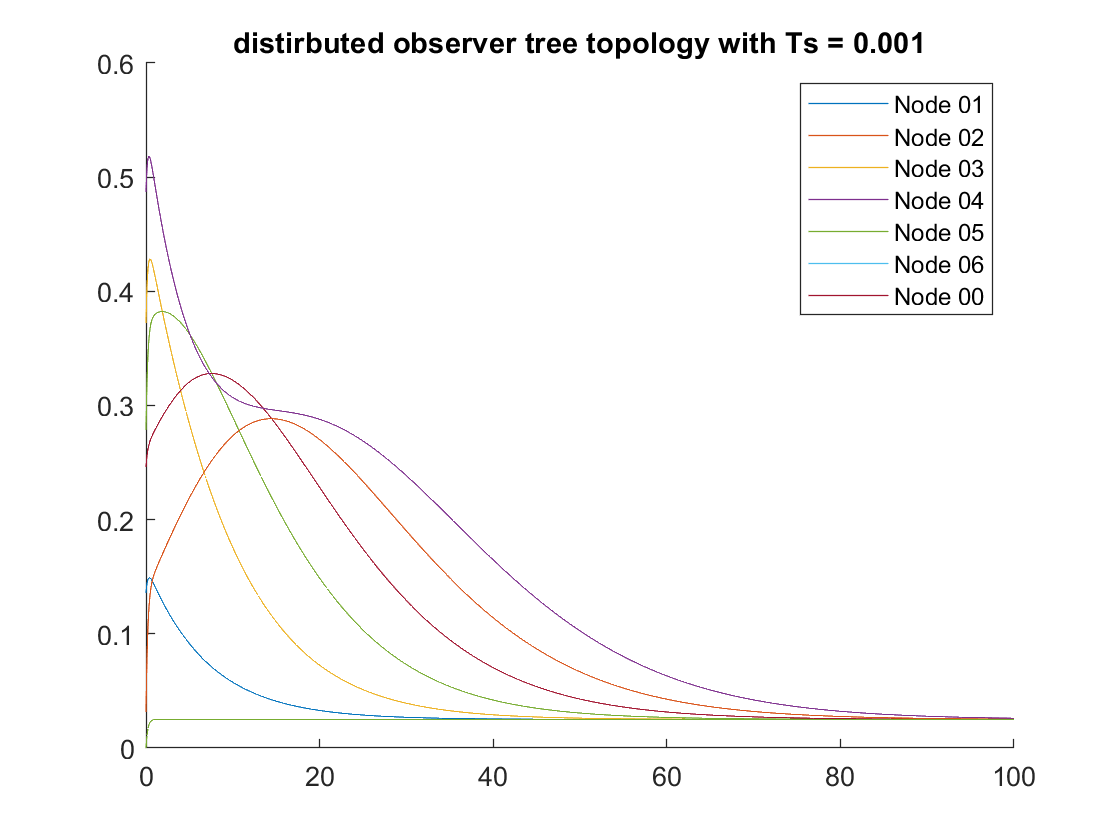
\includegraphics[width=0.50\textwidth]{tree_0.001.png} % Adjust width as needed
    \caption{The response of the nodes with the step reference in tree topology by discretized global observer with sampling time 0.001 second.}
\end{figure}

\begin{figure}[H] % h means "here", can also use t (top), b (bottom), p (page)
    \centering
    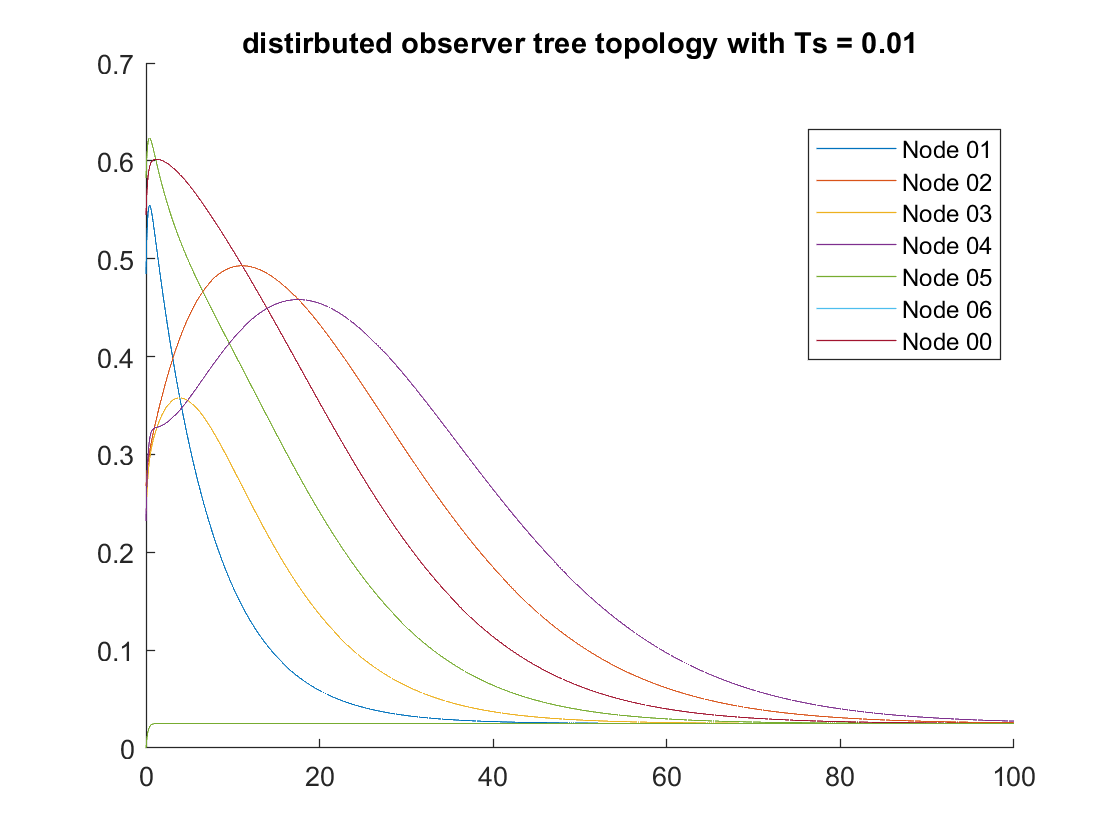
\includegraphics[width=0.50\textwidth]{tree_0.01.png} % Adjust width as needed
    \caption{The response of the nodes with the step reference in tree topology by discretized global observer with sampling time 0.01 second.}
\end{figure}

\begin{figure}[H] % h means "here", can also use t (top), b (bottom), p (page)
    \centering
    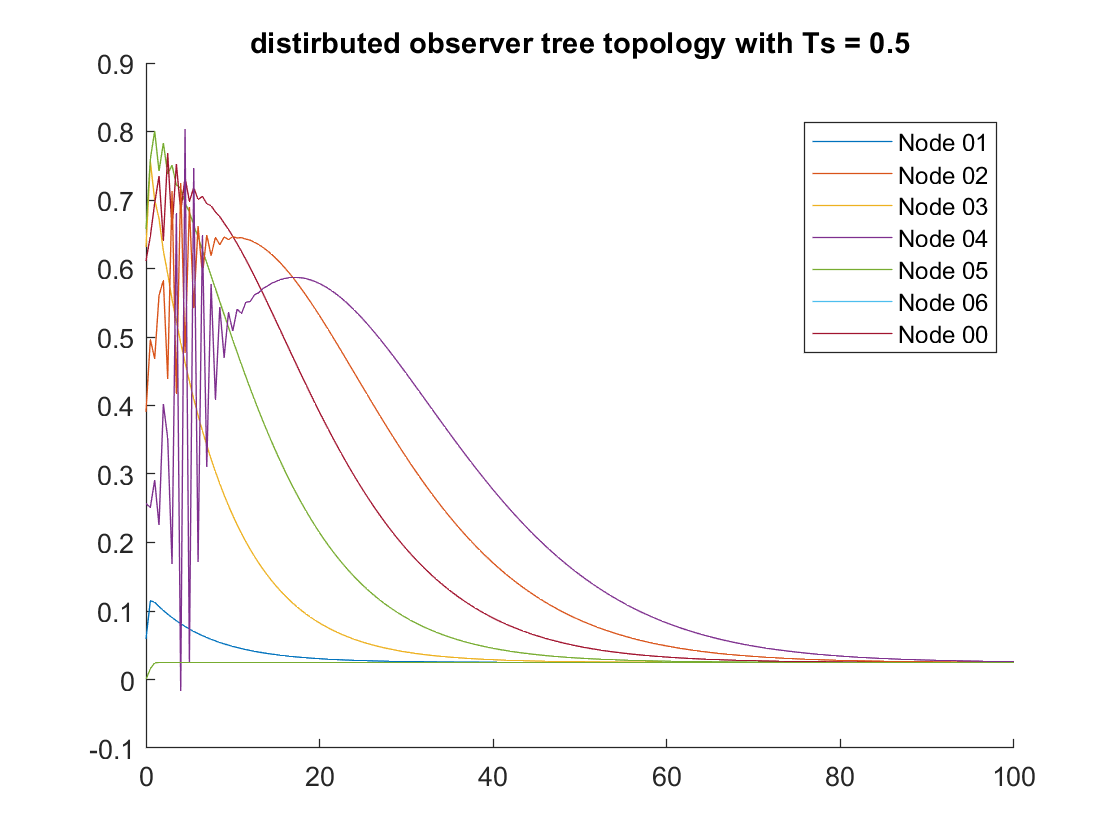
\includegraphics[width=0.50\textwidth]{tree_0.5.png} % Adjust width as needed
    \caption{The response of the nodes with the step reference in tree topology by discretized global observer with sampling time 0.5 second.}
\end{figure}



\section{The effect of the coupling gain $c$ and weight matrices $Q$ and $R$}
It can be seen that by increasing the coupling gain way larger than the threshold recommended by the theory, a better performance is obtained. In practice, nevertheless, it must be considered that using a large coupling gain is accompanied by large control input in the nodes, which depending on the size of the actuator, for relatively large values of coupling gain, saturation may be caused.

$Q$ is a diagonal matrix and it includes the weight of the states. By allocating weights to the states, it can be specified that which state is of higher importance for us.  $R$ is a diagonal matrix, and it include the weigh of the inputs. By increasing the value of $R$, the optimizer finds a solution that reduces the input effort as much as possible. 

It must be taken into account that improving performance is in conflict with reducing the input effort, and therefore, tunning these matrices is a matter of trade-off between these two objectives.


\section{Effect of noise}
Having investigated the effect of noise, it was realized that by increasing the coupling gain, the bound of the noise on the both states reduces, and this is correct also for the measurement noise. However, it seems counter intuitive, since it is expected that by increasing the value of the gain the effect of the noise accentuates.

\begin{figure}[H] % h means "here", can also use t (top), b (bottom), p (page)
    \centering
    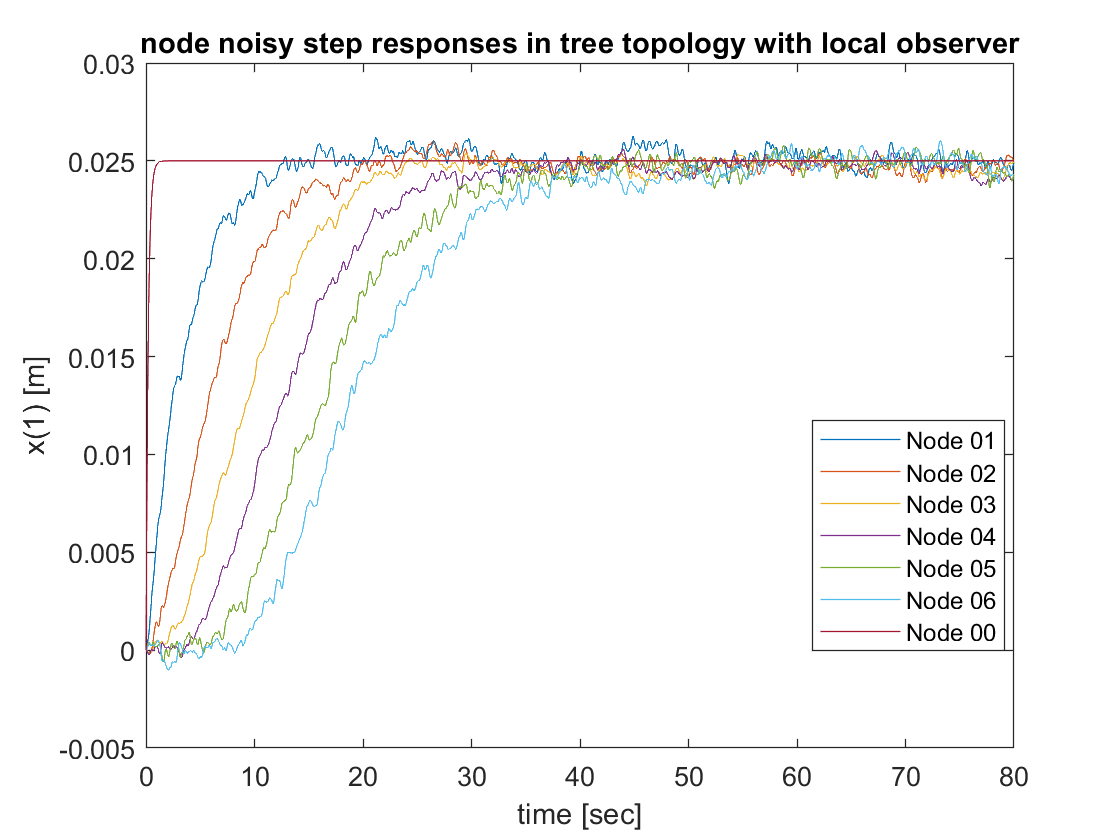
\includegraphics[width=0.50\textwidth]{noise1.png} % Adjust width as needed
    \caption{The simulation with noise;theoretical coupling gain plus one}
\end{figure}

\begin{figure}[H] % h means "here", can also use t (top), b (bottom), p (page)
    \centering
    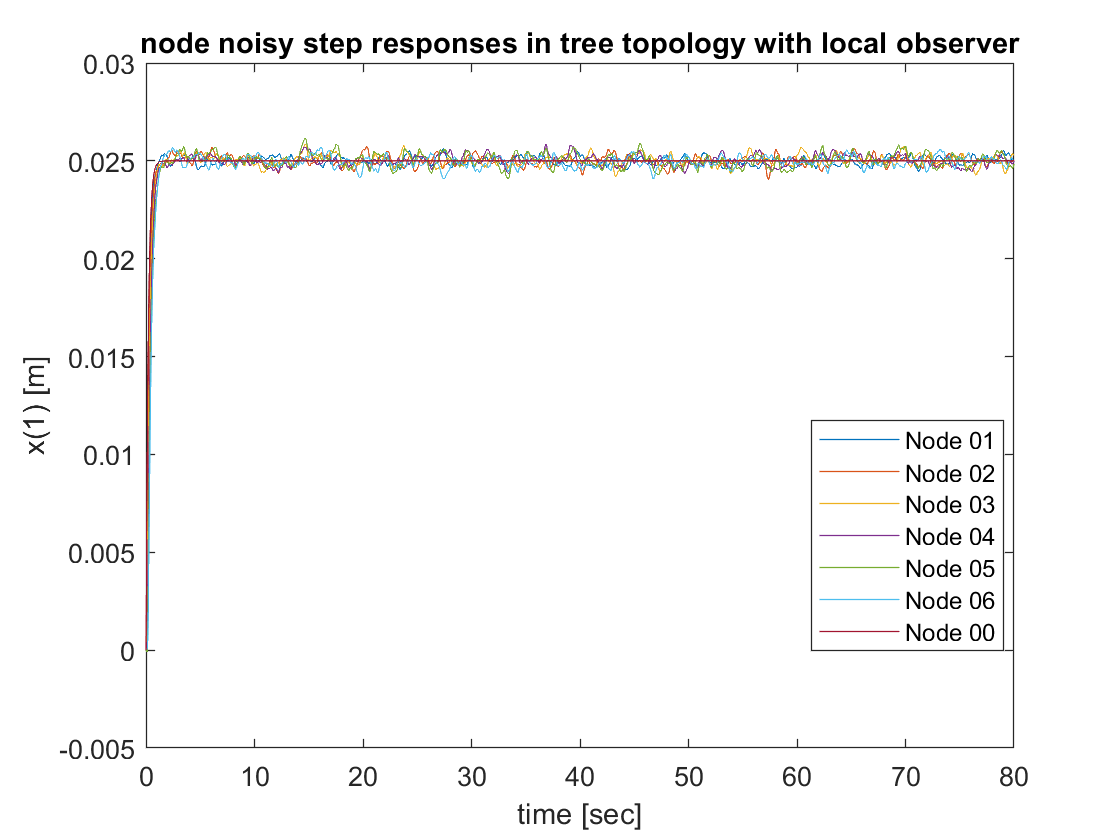
\includegraphics[width=0.50\textwidth]{noise100.png} % Adjust width as needed
    \caption{The simulation with noise;theoretical coupling gain plus one}
\end{figure}




%%%%%%%%%%%%

\section{Selected structure}
Since the nodes are originally unstable, and in practice, the communication between the noddes might not be idea, a local observer is prefered to guarantee the stability of the nodes under any communication channel condition. Further, given the suitable performance of star topology, a star topology is prefered to be used among the follower nodes.

